%\section{Introduction}

% \subsection{Goals of chapter and tools}

    In the previous chapter, I explored the possibility of a more robust typology of music notations such that we might more thoroughly assess the form and function of the twentieth century's thornier neo-notations. As a sort of a litmus test, this chapter will examine two work-complexes\footnote{Throughout this chapter, I use the term ``work-complex'' to describe clusters of works related by notational similarity. Unlike many bespoke notation schemes, the schemata I'll examine here have succeeded in persisting across multiple works in their artists' respective oeuvres. Specifically, though I'll predominantly be looking at Braxton's \textit{Composition No. 76} (1977) and Rădulescu's \textit{Das Andere} (1984), I consider \textit{No. 76} intimately bound up with related pieces such as \textit{Composition No. 98} and the majority of Braxton's Ghost Trance corpus--- similarly, \textit{Das Andere}'s notation scheme survives in Rădulescu's fifth string quartet, Op. 89 \textit{``before the universe was born''}.} by composers whose fascinating compositional practices and musico-philosophical commitments lie particularly close to my heart. The goals of the chapter are twofold: (1) to demonstrate the efficacy of the Ligetian typology in describing notation (and how we interact with it) in greater detail and (2) to gain novel insights into the works of Anthony Braxton and Horațiu Rădulescu via a more thorough reckoning with thus-far underappreciated aspects of their notation schemata.

% \subsection{Why Rad + Brax?}

    It goes without saying that these two artists represent two very distinct communities of practice; Braxton (b. 1945), a jazz-adjacent American composer/improviser known for incredibly variegated influences and tastes, and Rădulescu (1942--2008), a Romanian spectral composer renowned for his outsize personality and his pursuit of sound at the fringes of human psychoacoustic experience. As distinct as these backgrounds are, though, examining their scored works yields many fascinating parallels in the way they deploy dense, complex neo-notation in service of their musical aims. In contrast with many of the artists highlighted so far who have tended to stick to one neo-notational style, both Braxton and Rădulescu use notations across a wide gamut, including traditional and modified-traditional notations (both ``result'' and ``action''), novel signs which affect tightly-constrained ``micro-improvisation,'' relational symbols which constrain player gesture based on other performers' actions, and glyphs which provide uncoded spaces for improvisation based strictly on the performer's emotional state.

    The first section of this chapter will, with as little commentary as possible, catalog these works' signs according to their content and function, illustrating where they fall within our adopted typology. Following this, I will compare these two artists' chosen tools so as to illustrate the subtlety and complexity in the ways artists construct unique notions of openness in their respective works.
    
% \subsection{Why ``work-complex''?}
        

\section{Innovations in neo-notation}
   
\subsection[(\textit{Composition No. 76})]{$\vcenter{\hbox{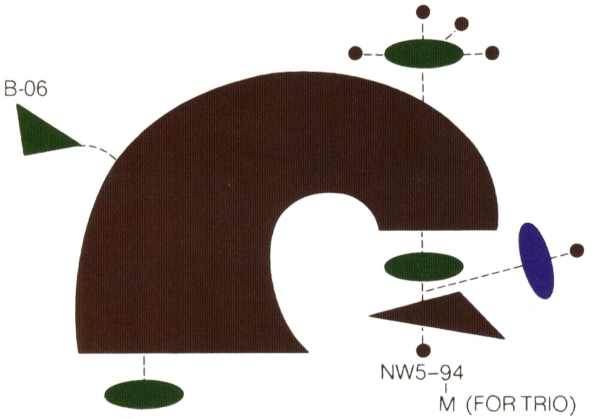
\includegraphics[width=3cm]{images/chapter3/comp76pictitle.png}}}$ (\textit{Composition No. 76})}

        Though Braxton's oeuvre comprises over 400 numbered works (at time of writing), each of them deserving a good deal more scholarly attention than they typically receive, \textit{Composition No. 76} (1977) merits singling out for a few reasons.\footnote{As is customary, I'll be referring to Braxton's works by their catalog numbers rather than by their proper graphic titles. While these titles (and especially their gradual change over the years) are fascinating in their own right, they unfortunately tend to typeset poorly. \textit{Composition No. 76}'s graphic title is given in the section heading.} First, only a relatively small number of his works have been formally published and made available to the general public---and many of these only relatively recently. Of these available works, \textit{No. 76} is by far the most complex in terms of its use of well-defined neo-notations and serves as a local apex in Braxton's musical and intellectual development during his flourishing in the mid-to-late 1970s. In contrast with the majority of individual pieces in Braxton's oeuvre, \textit{No. 76} has attracted some degree of scholarly attention owing, ostensibly, to the excerpted module used as the cover artwork for Braxton's seminal 1978 album \textit{For Trio}.\autocite{Braxton_For_Trio} Prior to widespread availability of Braxton's scores, scholars boldly assessed the work based primarily on speculation surrounding this single module. Finally, in 2018 Paul Steinbeck published ``Improvisation and Collaboration in Anthony Braxton’s \textit{Composition 76}''---likely the most thorough analysis yet of a single Braxton work---in an effort to rectify decades of incomplete scholarship.
    
        Braxton belongs to a rarefied class of musical innovators who consistently orient their artistry toward the future. Using the same working method we ascribe to, say, Miles Davis and Karlheinz Stockhausen, Braxton frequently develops a novel compositional practice seemingly from whole cloth and takes it to a sort of aesthetic conclusion before eventually beginning anew. As such, his works taken as a whole demonstrate an incredible diversity of sound- and process-concepts which are encoded via widely disparate methods. These range from complex, rigorously encoded but unscored solo works, to early post-Webernian works (his term) written entirely in traditional notation, to pieces in the much more recent ``Falling River Music'' scheme written predominantly with strictly connotative, asemantic painting and glyphs. \textit{No. 76} was written during a period in which Braxton consistently worked in several of these composition paradigms at once. As such, it displays a particularly dense, complex notation scheme, indebted to both American and European notational innovators like Cage, Feldman, Stockhausen, et al., as well as to the titans of Afrocentric improvised music on whose transcriptions Braxton cut his teeth.

    \subsubsection{Structure}

        Braxton has described \textit{Composition No. 76} in a number of different ways. One of my favorite synopses (taken from Braxton's five-volume \textit{Composition Notes} runs thus:

        \begin{smallquote}
            \textit{Composition No. 76} was conceived as an expanded context for three instrumentalists that attempts to provide terms for creative exploration. The reality of this form was conceived as a dynamic sound continuum that emphasizes the collective interchanges of its composite ensemble - rather than the `wonderful' soloist. [...]

            \vspace{7pt}

            \noindent To experience this work is not to hear a continuous succession of events - in the sense of events that flow from momentum into its next materialization (or `act') - rather in \textit{Composition No. 76} there is a static `dribble of isolated events that come together and apart without any sense of `applied' momentum (or `urgency'). This is a `lifeless' sound space that is somehow happening in spite of itself.\autocite[145-8]{Braxton_1988}
        \end{smallquote}
    
        For a more thorough grasp, one must look to the text of the score itself. Per its copyright page, \textit{Composition No. 76} is a trio for improvising multi-instrumentalists, comprising ``twenty-six pages of three-dimensional notation'' organized into 20 paired modules (labelled \{A1\}--\{A2\} through \{T1\}--\{T2\}\footnote{Mysteriously, a single module, \{E\}, contains three sub-modules; the first of which, \{E1\}, is composed only of a single whole note for Player 2.}) as well as seven pages of unison materials---also apparently modular---to be used in what Braxton dubs ``structural sequences'' throughout the performance.\autocite[149]{Braxton_1988} Though not given expressly in the score, it is clear from the pair of performances on \textit{For Trio} that module pairs may be performed in any order, though all three players take part in each module pair concurrently.
        
        As a brief illustration of performance proceedings, Figure~\ref{fig:a1a2} reproduces the first pair of modules, \{A1\}--\{A2\}---a typical arrangement throughout the piece.
    
                \begin{figure} 
                    \centering
                    \fbox{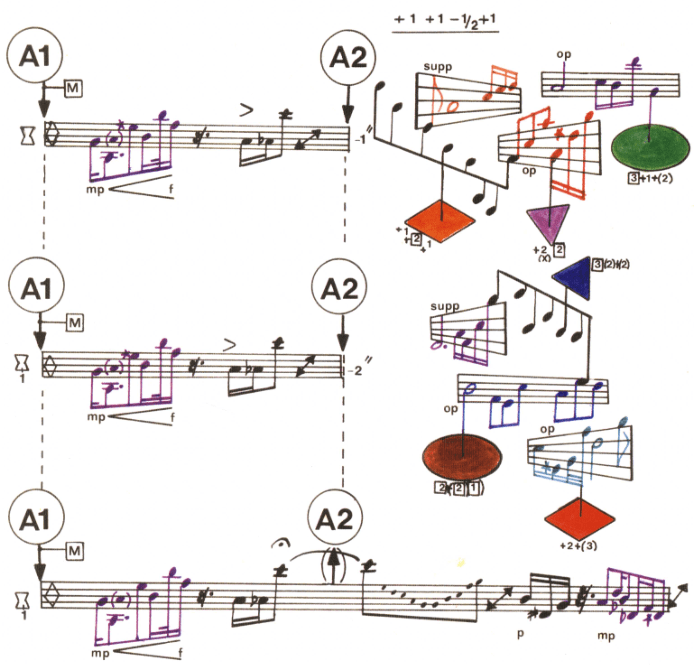
\includegraphics[width=.9\textwidth]{images/chapter3/a1a2.png}}
                    \captionsetup{width=.5\textwidth}
                    \caption[Module pair \{A1\}--\{A2\} from \textit{Composition No. 76}.]{Module pair \{A1\}--\{A2\} from \textit{Composition No. 76}.\footnotemark}
                    \label{fig:a1a2}
                \end{figure}
                    \footnotetext{\autocite[]{Braxton_1977}.}
    
        Over the course of each pair of modules, each player reads from left to right, either engaging in a more-or-less traditional fashion with the materials on standard staves (all three players in \{A1\}) or engaging with these seemingly opaque constellations of staff-fragments and geometric shapes as launchpads for constrained improvisation (players \#1 and \#2 in \{A2\}). The following section will be dedicated to a full unpacking of these materials so as to facilitate further discussion.
        % Though it may at first glance seem rather opaque, Braxton's detailed instructions allow \textit{No. 76} to be broken down into more graspable constituent glyphs. As an example, using the above figure as a reference and moving left to right on the page, we find:
    
        % \begin{smallquote}
        % \begin{enumerate}
        %     \item A bespoke glyph preceding \textbf{A1} indicating that all players are to match the instrument chosen by performer \#1
        %     \item A bespoke glyph indicating that all players are to match tempi
        %     \item The diamond clef ($\diamond$), Braxton's long-standing symbol which indicates that the following material may be read in any transposition
        %     \item Traditional dot-stem-beam notation in purple ink featuring fixed dynamics and the star accidental ($\star$) which stands in for either a sharp or a flat per the player's discretion.
        %     \item Traditional notation in black followed by Braxton's bespoke ``rest'' symbol, the diagonal double-headed arrow.
        %     \item A cue point at \textbf{A2}, whereupon two players enter into dense ``open material'' (to be discussed in greater detail anon.)
        % \end{enumerate}
        % \end{smallquote}
        
    \subsubsection{Braxton's fixed material}

        In Volume D of his 1988 \textit{Composition Notes}, Braxton describes \textit{No. 76} as fundamentally composed of ``fixed'' and ``open materials.'' As Steinbeck notes, though, these terms (at least under their typical usage) are essentially unable to fully capture the subtlety with which Braxton approaches his encoding scheme.\autocite[254]{Steinbeck_2018} Braxton seems to take this fundamental division between the ``fixed'' and the ``open'' quite seriously---to the point that his performance instructions are delivered across two pages: one dedicated to each primary category of notation. Table~\ref{tab:braxtoninstructions1} below reproduces in full Braxton's neo-notational glyphs used in this fixed material---featuring both his stated instructions as well as my categorization of each glyph according to the modified Ligetian typology established in the last chapter. The granularity with which Braxton's notation operates necessitates two new terms in describing these symbols: 
        
            \begin{smallquote}
                \begin{enumerate}
                    \item \textit{inducement}---a glyph which by itself invokes a certain FOP in a performer, leading to the execution of some gesture and a resultant sound. (We might take the traditional example: an individual note-head, which signifies that some action is to be taken to produce sound.)
                    \item \textit{modifier}---to contrast, a glyph which is used to modify some FOP by being appended to an inducement in one way or another. By itself (under normal circumstances) a modifier would not result in the performer taking any particular action---it is only when appended to a sounding glyph that a modifier can affect sonic results. (For example: the flags, beams, dynamic markings, and articulations which accompany the note-head).
                \end{enumerate}
            \end{smallquote}
       
        As seen in the previous chapter with Braxton's early ``Ghost Trance'' notation, it is possible to deploy a highly stripped-down notation scheme---that is, one which eschews most modifiers in favor of only barely-adorned inducements. In this case, Braxton seeks to deliberately leave the bulk of the parameters normally described by a more full-featured notation up to the performer and thus omits those glyphs which would typically delineate said parameters. Nevertheless, ``Ghost Trance Music'' as well as every other notation scheme examined here (result, action, recipe, et al.) can be meaningfully described as some arrangement of various inducements and modifiers. Using these definitions, Table~\ref{tab:braxtoninstructions1} presents and describes each novel symbol given on \textit{Composition No. 76}'s first page of instructions. 
        
        %As demonstrated in the previous chapter, semantically coherent systems of notation can be deployed which use barely-adorned inducements---necessarily very loosely constrained insofar as they do not feature the typical modifiers which would accompany them in traditional notation. However, under every coherent notation scheme we've encountered thus far, any of the notational sub-types (result, action, recipe) may comprise many different inducements and modifiers---and as we will see given Braxton's detailed instruction set, this scheme is no exception.

   % Despite the wide latitude granted to performers, per Braxton's understanding everything preceding \textbf{A2} is considered ``fixed material.'' Insofar as the symbols involved in are concerned, I have taken the liberty of reproducing the table provided with the instructions below in full for ease of reference in~\ref{tab:braxtoninstructions1}.
    
    
        \begin{table}
        \NewTableCommand\myhline{\hline[0.1em]}
            \scriptsize
            \centering
            \singlespacing
                \begin{tblr}{
                cells={valign=m, halign=l},
                width=\textwidth,
                colspec={l X[2.5] X[1] X[-5]},
                column{3}={halign=c}
                }
                    \myhline
                    & \textbf{Instruction given} & \textbf{Symbol} & \textbf{Comment}\\ [0.5ex]
                    \myhline
                    \textbf{1.} & ``Match dynamics'' 
                        & $\vcenter{
\includegraphics[width=1cm]{images/chapter3/instructions/01.png}}$ 
                        & Relational, interpersonal. Recipe, modifier. Constrains dynamics. \\
                    \textbf{2.} & ``Match dynamics but very softly'' 
                        & $\vcenter{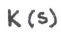
\includegraphics[width=1cm]{images/chapter3/instructions/02.png}}$ 
                        & (as above) \\
                    \textbf{3.} & ``Play note then improvise for small amount of time'' 
                        & $\vcenter{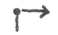
\includegraphics[width=1cm]{images/chapter3/instructions/03.png}}$ 
                        & Recipe, inducement. No appreciable constraint. \textit{Appears in instructions but not in score.}\\
                    \textbf{4.} & ``Hold until next cue point (suspension)'' 
                        & $\vcenter{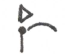
\includegraphics[width=1cm]{images/chapter3/instructions/04.png}}$ 
                        & Relational, interpersonal. Recipe, modifier. Fixed based on prior action taken. \\ 
                    \textbf{5.} & ``Prepare just before time cue (and then execute)'' 
                        & $\vcenter{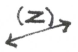
\includegraphics[width=1.5cm]{images/chapter3/instructions/05.png}}$ 
                        &  Modifier. Restricts onset time for execution of phrase.\\
                    \textbf{6.} & ``Cue for someone else [...]'' 
                        & $\vcenter{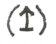
\includegraphics[width=1cm]{images/chapter3/instructions/06.png}}$ 
                        & Strictly informational. Orients performer with regard to other events in the score. \\
                    \textbf{7.} & ``Can be used for vocal phrase'' 
                        & $\vcenter{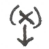
\includegraphics[width=1cm]{images/chapter3/instructions/07.png}}$ 
                        & Modifies improvisatory inducements. Relaxes constraint by expressly permitting vocal execution.\\
                    \textbf{8.} & ``Wait for near the end of the time group to finish phrase point [...]''
                        & $\vcenter{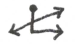
\includegraphics[width=1.5cm]{images/chapter3/instructions/08.png}}$
                        & Relational, contingent on elapsed time. Recipe, modifier.\\
                    \textbf{9.} & ``Rest'' 
                        & $\vcenter{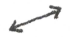
\includegraphics[width=1.5cm]{images/chapter3/instructions/09.png}}$
                        & Result notation (silence), inducement. Duration potentially contingent on other players' actions.\\
                    \textbf{10.} & ``Match instrument (that principle figure in time zone is playing) [...]''
                        & $\vcenter{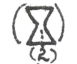
\includegraphics[width=1cm]{images/chapter3/instructions/10.png}}$
                        & Relational, interpersonal. Recipe, instrumental constraint. Modifier.\\
                    \textbf{11.} & ``Change dynamics abruptly for next playing section [...]'' 
                        & $\vcenter{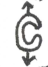
\includegraphics[width=.7cm]{images/chapter3/instructions/11.png}}$
                        & Relational, self. Recipe, dynamic constraint. Modifier. FOP excludes prior dynamic attributes.\\
                    \textbf{12.} & ``Rest for 3 to 5 seconds'' 
                        & $\vcenter{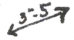
\includegraphics[width=1.5cm]{images/chapter3/instructions/12.png}}$
                        & Result notation (silence), inducement. \\
                    \textbf{13.} & ``Change instrument quickly'' 
                        & $\vcenter{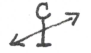
\includegraphics[width=1.5cm]{images/chapter3/instructions/13.png}}$
                        & Relational, self. Recipe, instrumental constraint, modifier.\\
                    \textbf{14.} & ``Independent tempo'' 
                        & $\vcenter{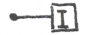
\includegraphics[width=1.5cm]{images/chapter3/instructions/14.png}}$
                        & Relational, interpersonal. Recipe, tempo constraint, modifier. Unclear if tempo \textit{must} be distinct or merely ``uncoupled''.\\
                    \textbf{15.} & ``Match tempo [...]'' 
                        & $\vcenter{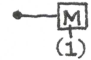
\includegraphics[width=1.5cm]{images/chapter3/instructions/15.png}}$
                        & Relational, interpersonal. Recipe, tempo constraint, modifier.\\
                    \textbf{16.} & ``Open clef'' 
                        & $\vcenter{
\includegraphics[width=.7cm]{images/chapter3/instructions/16.png}}$
                        & Modifier. Relaxes constraint on phrase execution by incorporating transposition into FOP.\\
                    \textbf{17.} & ``Sharp or flat'' 
                        & $\vcenter{
\includegraphics[width=.7cm]{images/chapter3/instructions/17.png}}$
                        & Modifier. Relaxes constraint on note execution by incorporating transposition into FOP.\\
                    \myhline
                \end{tblr}
        \captionsetup{width=.5\textwidth}
        \caption[Composer-provided list of symbols from Braxton's \textit{Composition No. 76}]{Composer-provided list of symbols from Braxton's \textit{Composition No. 76}.\footnotemark}
        \label{tab:braxtoninstructions1}
    \end{table}
        \footnotetext{\autocite[instructions pg. 1]{Braxton_1977}.---Index numbers in this case correspond with those provided in the score.}

       Fixed notation in \textit{No. 76} might be thought of as a heavily-modified form of traditional notation insofar as it features (1) traditional ${time}\times{pitch}$ mapping on the $x$- and $y$-axes; (2) (some) traditional clef indications; (3) phrases expressed using the dots, stems, and beams of traditional notation; and (4) other traditional modifiers such as dynamic markings, articulations, and fermate. 
    
       This is by and large the extent to which Braxton imports familiar symbols. However, certain neo-notational glyphs replicate or tweak traditional functions despite their novel form. The new clef (16.) and new accidental (17.) (both long-time Braxton staples) in essence serve the same purpose as their familiar counterparts, merely adding another degree of openness to the score's realization by reducing constraints typical to a given musical passage. The bespoke symbol for ``rest'' (without modifier at 9. and with duration indication at 12.) simply serves as a proportional stand-in for typical absolute-duration rests. Likewise, while Braxton's new cuing symbols (5. and 6.) fill an important role in that they aid players in orienting themselves within material, they ultimately replicate functions available in traditional notation as well. (Color, insofar as it is featured in fixed material, also serves a ``tweaked'' traditional role, though I'll expand on this in a coming section.)
       
       We also find, however, that Braxton employs many symbols which fulfill roles not typically found in traditional notation. Specifically, his novel relational symbols serve as important additions for a music which seeks to systematically constrain improvisers' creative output. That is to say: instructions 1., 2., 4., 8., 10., 11., 13., 14., and 15. all serve to mediate a performer's actions not based on a desired sonic product per se (i.e. some absolute factor) but instead based on the \textit{relation} between the player and some other variable---either another player's actions (as in the ``match dynamics'' or ``match tempo'' indications) or one's own prior decisions (``change instrument quickly'' or ``change dynamics abruptly''). In both of these cases, the final outcome results from a confluence of an individual player's choices, all players' actions as a group, and the composer's meta-constraints established pre-performance.
    
       Of course, relational parameters are not exclusive to neo-notation. Dynamic markings and expressive texts found in traditional notation tacitly rely on relational parameters. For example, when I read \textit{ritardando} the precise rate of my slowdown depends upon that of my stand-mate. Likewise, the increase in amplitude from \textbf{\textit{p}} to \textbf{\textit{f}} is contingent on the loudness of my initial expression. However, symbols like Braxton's \#8., 14. or 15. which \textit{deliberately} (rather than incidentally) parametrize the gestures and sonic products of other performers are essentially foreign to the encoding schemes familiar to most musicians. Here, Braxton is making explicit what were predominantly implicit characteristics of prior notations.
    
    \subsubsection{Braxton's open material}

            \begin{figure} 
                \centering
                \fbox{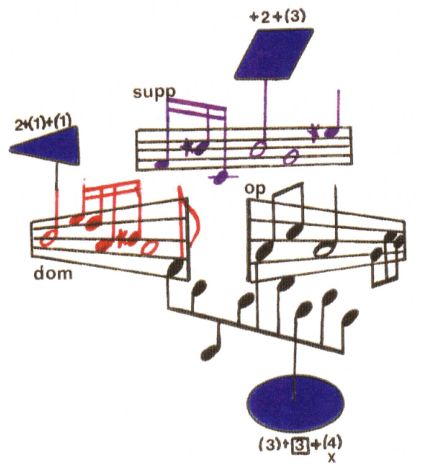
\includegraphics[width=.4\textwidth]{images/chapter3/openf1.png}}
                \captionsetup{width=.55\textwidth}
                \caption[Open sub-module \{F1\} from \textit{No. 76}.]{Open sub-module \{F1\} from \textit{No. 76}.\footnotemark}
                \label{fig:openf1}
            \end{figure}
                \footnotetext{\autocite[]{Braxton_1977}.}
            
        \textit{No. 76}'s open material is easily distinguishable by spatial separation (``floating'' on the page without being tethered to a single staff) and by its geometry. Here we find the three-dimensionality Braxton referenced earlier: staves in open material are fragmentary and clef-less; seeming to emerge from and recede into the page as though they were two-dimensional projections of massy objects in space. Though now accompanied by constellations of modifier symbols, play is still oriented around these staff fragments, which may be approached non-linearly: that is, in any order. Per Graham Lock, it appears that an adequate realization of these sub-modules requires that each staff-fragment be interpreted, though in no particular order.\autocite[Postscript 3]{Lock_1989}
    
        In practice, a single ``unit'' of open notation consists of a staff-fragment in some orientation (implying a particular positionality in three-dimensional space). Notes inscribed on these staff-fragments typically appear in color, though they may also be rendered in the traditional black. Almost universally, these staff fragments are modified by an attached simple geometric shape filled with color. These appear to the reader to be ovals (full or truncated), irregular triangles, and skewed quadrilaterals, but are almost certainly intended to be equilateral triangles, squares, and circles subjected to the same system of projection as the staff fragments. Modifying these colored shapes are short sequences of numeric code. Finally, each open sub-module features one or more ``linking'' gestures comprising staffless eighth-note figures in black which share stems with two staff fragments (as shown above in Figure~\ref{fig:openf1}). 

        All explicit instructions pertaining to open material are given on the second instruction page and are reproduced in Table~\ref{tab:braxtoninstructions2} below. 

        \begin{table}
        \scriptsize
        \centering
        \singlespacing
            \begin{tblr}{width=.8\textwidth, colspec={l X[2.5] X[-2.5]}}
                \hline[0.1em]
                 & \textbf{Information} & \textbf{Note} \\ 
                \hline[0.1em]
                \textbf{A.} & $\vcenter{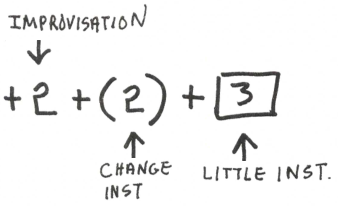
\includegraphics[width=4cm]{images/chapter3/instructions/instA.png}}$
                    & $\vcenter{Numbers indicate number of notes/phrases per improvisatory sub-module (?). They may be modified with parentheses or squares.}$\\
                \textbf{B.} & $\vcenter{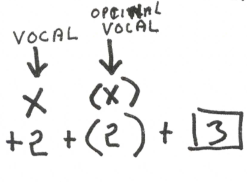
\includegraphics[width=3cm]{images/chapter3/instructions/instB.png}}$
                    & $\vcenter{Improvisatory indices may also be modified with $\times$ or $(\times)$ indicating mandatory or optional use of vocals for improvisation.}$\\
                \textbf{C.} & $\vcenter{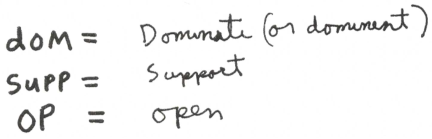
\includegraphics[width=5cm]{images/chapter3/instructions/instC.png}}$
                    & $\vcenter{Relational signifiers orienting improvisation in one of three ways with regard to other performers.}$\\
                \textbf{D.} & $\vcenter{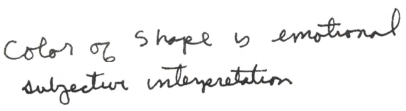
\includegraphics[width=5cm]{images/chapter3/instructions/instD.png}}$
                    & $\vcenter{Expressly indicates presence of performer-mapping as critical component of performance.}$\\
                \hline[0.1em]
            \end{tblr}
            \captionsetup{width=.5\textwidth}
        \caption[Supplementary instructions from Braxton's \textit{Composition No. 76}.]{Supplementary instructions from Braxton's \textit{Composition No. 76}.\footnotemark}
        \label{tab:braxtoninstructions2}
            \end{table}
                \footnotetext{\autocite[instructions pg. 2]{Braxton_1977}.---Note that Braxton opts not to concretely define the fundamental unit of improvisatory action signified by the numeric code. Steinbeck claims it might refer either to notes or phrases.}

        As is clear from the given instructions, Braxton's open material is still subject to rather stringent restrictions. In its execution, open material is divided into clusters of improvised gestures induced by each staff-fragment/shape combination. These clusters comprise a rendering of the modified-traditional notation within the staff-fragment as well as a series of notes or phrases delimited by the codes of the form \{$+\:i + j +... + n$\}. Parenthetical or square modifiers indicate a change of instrument in between soundings or the use of the AACM signature ``little instruments'', respectively.\footnote{\autocite[170]{Jost_1994}.---A ``little instrument'' is a (typically small) auxiliary percussion or wind instrument deployed to add color or break up the prevailing texture. These include but are not limited to ``slide whistles, recorders, harp, Japanese koto, harmonica, kazoo, police whistles, thunder sheet, bells and gongs, plus countless other percussion instruments.''} Elements of the numeric code may be accompanied by $\times$ or $(\times)$, indicating mandatory or optional use of the voice in the specified improvisation-group.
    
        Open material features its own bespoke relational signifiers. \textsc{dom}, \textsc{supp}, and \textsc{op} indicate that an improvisatory cluster should either dominate, support, or remain un-coupled from the prevailing ensemble texture. These are distinct from the ``fixed'' relational symbols in that they demand significantly more creative interpretation---i.e. restrict a performer's FOP much less. Where ``match dynamics'' or ``change instrument quickly'' are rather straightforward in their interpretation and feature very little ambiguity, \textsc{dom} and \textsc{sup} modifiers are not merely functions of greater/lesser dynamic or density. Rather, they require a performer to assess in-the-moment the sort of gesture which befits a given sonic environment from among an essentially infinite array of potential actions.

    % \begin{notestuff}
    %     This verges on too much commentary for this dry, explanatory section---I'm gonna return to it later.
    % \end{notestuff}

        Braxton's distinct use of color in \textit{No. 76} almost certainly accounts for a significant portion of interest (scholarly or otherwise) in the score. Per Table~\ref{tab:braxtoninstructions2}, the only instruction explicitly given in the text with regard to color is the rather vague pronouncement that ``color of shape is emotional subjective interpretation.'' Of course, colored inks not only appear in the geometric figures, but were used to inscribe both open and fixed phrases as well. Graham Lock, perhaps the most widely-read Braxton scholar, describes the intentions behind this color scheme in a footnote:
        
            \begin{smallquote}
                The colour code to \textit{Composition 76} is actually based on astrological correspondences. That is, Braxton selected a set of the emotional characteristics attributed to various signs of the zodiac and then designated them in the score by using the colours associated with the same signs. The code is: blue = sombre or moody (Saggitarius); red = explosive or intense (Aries); green = calm, restrained or contained (Taurus); violet = vibrant or pulsing or energetic or vigorous (Pisces); brown = complementary or harmonious or balancing (Libra); yellow = strong, lyrical or bright (Leo).\autocite[222]{Lock_1989}
            \end{smallquote}
        
        In a related 2008 paper, Lock reiterates much of the same information but adds:
        
            \begin{smallquote}
                Shades of colour mark factors such as dynamic and tempo: the darker the hue, the faster and/or louder you play.\autocite{Lock_2008}
            \end{smallquote}
    
        That Braxton opts not to disclose this important scheme in the text of his score is interesting in and of itself and will be revisited in a later section. For now, though, it suffices to say that taken whole, the graphic elements in his open material are neither fully denotative nor fully connotative. If we take the code given by Lock at face value, color inside shapes (and presumably when applied to traditional notation as well) serves essentially as once-abstracted expressive text which applies to a given improvisatory expression; a stripped-down rendering of instructions of the form ``\textit{con eleganza},'' ``\textit{molto agitato},'' ``\textit{doloroso},'' etc. Clearly, however, certain aspects of these signs remain un-coded. The shapes' forms, for instance; their precise positioning relative to the staff fragments; the virtual orientation of the staff fragments themselves with respect to the viewer---each of these factors poses a ``graphical excess'' connoting additional factors which appear to be strictly performer-mapped.\footnote{\autocite{Dicker_2016}.---These symbols recur frequently throughout Braxton's oeuvre and are discussed at length (independent of any one composition) in his \textit{Tri-Axium Writings} and elsewhere. They make their most prominent appearance in his later ``Ghost Trance Music'' composition series, where they serve as ``jumping-out'' points where performers leave the prevailing (written) musical material to improvise before returning at another iteration of the same symbol. Triangle, square, and circle correspond to, respectively: ``synthesis or correspondence logics;'' ``stable logics;'' ``mutable logics.''}
    
        Worth noting is that at a base level, Braxton's open notation functions much in the same way as his fixed material: i.e. by providing sequences of inducements flanked by various modifiers. This is very much not a given for other forms of un-coded open notation, which may well bundle together graphic elements in such a way that individual glyphs are impossible to parse as providing any one particular function (e.g. Cardew's inscriptions in \textit{Treatise} discussed last chapter).

        % \begin{notestuff}
        %     This raises a very important point about the notion of ``completeness'' of representation of sound- or process-concepts in the written score. It seems like the 19th-century ``Eurological'' model would always have it that the composer's S/PCs should be represented as entirely as possible in the written score, while for Braxton this is obviously not the case. This merits a good bit of discussion in the comparative section!
        % \end{notestuff}

    % \begin{uselater}
    % \begin{smallquote}
    %     The musician can enter the module at any point, and go around it in any direction. ... All primary shapes (circle, triangle, oblong etc.) are in colour (as is some of the notation) and designate improvisation, the different colours and shapes indicating the kinds of improvisation to be played ... \autocite[Postscript 3]{Lock_1989}
    % \end{smallquote}
    % \end{uselater}

    \subsubsection{Unknowns}

        Despite its position as one of Braxton's most-discussed works (and despite Braxton's own commentary in his \textit{Composition Notes}), certain notational elements still remain fundamentally opaque; either by design or because of incomplete knowledge on the part of its analysts. For completeness' sake, I'll reproduce these here in Table~\ref{tab:mysteryglyphs}.

            \begin{table}
                \footnotesize
                \centering
                \singlespacing
                    \begin{tblr}{width=.7\textwidth, colspec={l X[2.5] X[-3.5]}}
                        \hline[0.1em]
                         & \textbf{Information} & \textbf{Note} \\ 
                        \hline[0.1em]
                        \textbf{1.} & $\vcenter{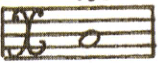
\includegraphics[width=2.5cm]{images/chapter3/mystery01.png}}$
                            & $\vcenter{``Mirrored-C'' or ``$\mathscr{X}$'' clef which occurs sporadically throughout the score.}$\\
                        \textbf{2.} & $\vcenter{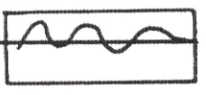
\includegraphics[width=2.5cm]{images/chapter3/mystery02.png}}$
                            & $\vcenter{Action notation in the form of sinusoidal line in structural sequences.}$\\
                        \textbf{3.} & $\vcenter{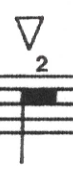
\includegraphics[width=1cm]{images/chapter3/mystery03.png}}$
                            & $\vcenter{Rectangular notehead in structural sequences.}$\\
                        \textbf{4.} & $\vcenter{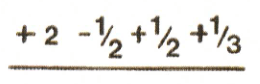
\includegraphics[width=4cm]{images/chapter3/mystery04.png}}$
                            & $\vcenter{Example of additional numeric code appended to each open sub-module. Not to be confused with improvisation modifiers shown in Table~\ref{tab:braxtoninstructions2}.}$\\
                        \hline[0.1em]
                    \end{tblr}
                    \captionsetup{width=.5\textwidth}
                \caption[Glyphs of unknown significance in \textit{Composition No. 76}.]{Glyphs of unknown significance in \textit{Composition No. 76}.\footnotemark}
                \label{tab:mysteryglyphs}
            \end{table}
            \footnotetext{\autocite{Braxton_1977}.}

        Listening to the two ``canonical'' extant recordings yields some insight. First: A simple whole-note figure using the un-referenced ``mirrored-C'' or ``$\mathscr{X}$'' clef results in distinct chords in the two versions (shown below in Figure~\ref{fig:mysteryclef}). A fair assumption might be that the clef serves as a yet more open version of the diamond clef where onset and duration are relatively fixed and precise pitch is held open. This seems to be confirmed by Tri-Centric Foundation Archives manager Carl Testa, who, in reference to a sketch of the much-earlier \textit{Composition No. 6E} (1968), writes that ``[t]he score features an ``X'' clef which indicates to the performers that exact pitch reproduction is not required [...]'' (though the glyphs do not match precisely).\autocite{Testa}

            \begin{figure}
                \centering
                \subfloat[\centering in score]
                {{\fbox{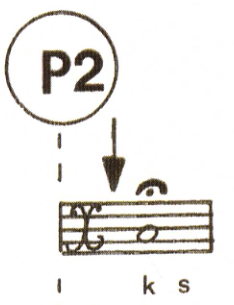
\includegraphics[width=.18\textwidth]{images/chapter3/moduleP2mysteryclef2.png} }}}%
                \qquad
                \subfloat[\centering transcription (conc.)]{{\fbox{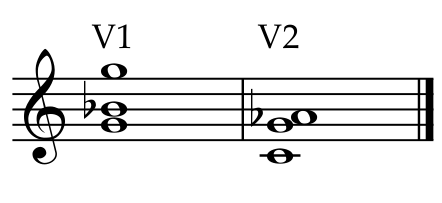
\includegraphics[width=.3\textwidth]{images/chapter3/moduleP2mysteryclef.png} }}}%
                \captionsetup{width=.55\textwidth}
                \caption[``Mirrored C'' or ``$\mathscr{X}$'' clef at sub-module P2 in V1/V2 on \textit{For Trio}.]{``Mirrored C'' or ``$\mathscr{X}$'' clef at sub-module P2 in V1/V2 on \textit{For Trio}.\footnotemark}%
                \label{fig:mysteryclef}%
            \end{figure}
            \footnotetext{\autocite[2:27-3:18 of Version 1 and 4:44-6:03 of Version 2]{Braxton_For_Trio}.}

        Next: The sinusoidal line typically reserved to signify trills in other works seems to indicate open improvisation with a duration limited by cues. Performances on the album render this symbol using rapid switches between instruments, long tones, short bursts of sound, etc., and vary considerably in length. The rectangular notehead (resembling the \textit{maxima} from medieval/Renaissance mensural notation) occurs infrequently, but seems to be rendered simply as a slightly longer quarter-note pulse. Lastly and perhaps most mysteriously: I can find no reference to the ``secondary'' numeric codes which appear appended to each open sub-module. Unlike their coded counterparts which describe attributes of improvisatory ``clusters,'' numbers in these secondary codes appear signed (either ``$+$'' or ``$-$'') and include fractional values---neither of which pertain to the prior code given above in Table~\ref{tab:braxtoninstructions2}. Again, as is often the case in Braxton's work, it remains unclear whether these symbols' lack of well-defined function (at least as explained in the score) serves as a deliberate omission or an oversight, or whether perhaps their function was so clear to the participants as to have made their explicit definition unnecessary. I will return in greater detail to this notion in a later section.

            \begin{center}
            \vspace{-10pt}
            \noindent\rule{3cm}{0.4pt}
            \end{center}

        % WRAP-UP PARAGRAPH
        Thus, an individual performance of \textit{Composition No. 76} proceeds as follows: Pre-performance, performers decide upon a particular ordering of module-pairs and fixed structural sequences. In executing these module-pairs, players seamlessly slip between engagement with more restricted linear interpretation of fixed materials and omnidirectional interpretation of open materials; all the while maintaining certain temporal, dynamic, and structural relations with regard to other performers. Though Braxton thinks of these fixed and open performance paradigms as distinct modes of play, it's clear from examining the notation that this distinction is, in the end, quite blurry.
    
        Before moving on to discuss the import of Braxton's notational choices, however, I would like to pivot rather abruptly to another work-complex by an unlikely kindred spirit---one in whose work we'll see many noteworthy parallels and perpendiculars.
    
\subsection{\textit{Das Andere} \& Op. 89 \textit{``before the universe was born''}}

        In contrast with other composers willingly or unwillingly linked to the spectralist paradigm, Horațiu Rădulescu has, for a variety of reasons, received considerably less scholarly attention. Known among fans and detractors alike for his outsize personality, his ``convoluted, jargon-heavy writing'', and most of all for his highly idiosyncratic sound worlds, Rădulescu parallels Braxton insofar as he is often seen as an ``outsider'' in his field.\autocite{Suckling_2018} More than anything else, Rădulescu's particular flavor of spectralism is characterized by a fascinating form of sonic indeterminacy he dubs \textit{sound plasma}. So dense and poly-timbral as to resist traditional descriptors, \textit{sound plasma} comprises a range of techniques including ``sparkling, irregular trill[s],'' ``irregular arpeggios [...] with extreme \textit{flautando} bowing,'' and ``irregular, breathy `phase shifting' timbre[s],'' all of which combine in myriad ways to (ideally) produce the galaxies of resultant sum and difference tones which Rădulescu seeks.\autocite{Heery_2016}
                
        This section concerns a work-complex comprising two of Rădulescu's compositions, \textit{Das Andere} (1984) and Op. 89, \textit{``before the universe was born''} (1995), for unaccompanied viola and string quartet, respectively---two pieces which epitomize his pursuit of this elusive \textit{klangwelt}. For R\u{a}dulescu, \textit{Das Andere} represented an early attempt to solve the problem of adapting plasmatic music---usually reliant on complex, chaotic interactions between multiple sounding bodies---to a single instrument\autocite[10]{Marinescu}  To that end, he developed a fascinating, singular notation scheme to facilitate his measured indeterminacy. Evidently, this experimental foray was successful enough that he continued to deploy elements of \textit{Das Andere}'s notation throughout his career (albeit with various mutations), including in Op. 89.\footnote{This fact is noteworthy in and of itself given that experimental notations typically fail to live past the age of a single piece.} 

        Of R\u{a}dulescu's predilection for new notations, Liviu Marinescu explains:

            \begin{smallquote}
                [...] his desire to notate differently came from the need to compose differently. [...] For centuries, the Western world had worked slowly on developing a notation system that removed approximation between what was seen, what was played, and what was ultimately heard. Horațiu Rădulescu saw this old routine as a significant obstacle in the creation of plasmatic music, which is why he sought to return much of the initiative and creative power back to the performer.\autocite[1]{Marinescu}
            \end{smallquote}

        \noindent In the following sections, I will demonstrate precisely how and to what extent R\u{a}dulescu was able to achieve this ``transfer'' by closely examining the unique notational syntax and semantic content developed for these two pieces.

    \subsubsection{Rădulescu's notation scheme---denotative factors}
        
        Notation in \textit{Das Andere}/Op. 89 is a form of \textit{tablature}---a subset of action notation which encodes actions pertaining to the relationship between player and instrument-body.\footnote{This is to say: per Chapter 2, syntactic relations between signs in tablatures do not map to resultant sounds in the same way they would in result notations like our traditional pitch-centric notation.}. \textit{Das Andere} (being the simpler case) features staff lines representing the four strings of the viola, arranged from high to low.\footnote{
            To be precise, Instruction pg. 1 subtitles the piece ``for a stringed instrument tuned in perfect fifths.'' R\u{a}dulescu has since published an alternate score for 'cello which he also suggests be used for violin or double bass.
            } 
        As in traditional guitar/lute tablatures, most symbols used in Rădulescu's system reflect positions for the player's left hand. Unlike guitar tablature, however, where fret positions represent the subdivision of a particular string into sectors allowing for pitches in 12-tone equal temperament, numeric position values in Rădulescu's works most often represent the locations of natural harmonics on the string. For instance, a ``7'' on the uppermost staff line would indicate that the player ought to place a finger at the 7th-harmonic position on string I of the viola. Also unlike traditional tablature, this position marker by itself does not signify a particular sounding---as when one plucks a harmonic on guitar incited by ``$\diamond$'', for example. Rather, \textit{Das Andere} and Op. 89 feature specific sets of actions meant to sound these harmonics in different ways. 
    
        There are two primary sets of actions Rădulescu employs in the pieces (which he analogizes as ``play characters'' in his supplementary material represented by \textit{alpha} ($\newalpha$) and \textit{sigma} ($\Upsigma$) in the score.\autocite[dedication page]{Radulescu_1984} Given that these function as mutable, flexible notations which themselves might be modified by subsidiary symbols, I think of these as ``second-order'' notations which cluster together complex performance parameters into comparatively neat packages; much in the way that the baroque ``turn'' reduces a complex set of actions down to a single glyph, which itself is modified by key signature, tempo, meter, etc.
    
        In a series of instruction pages provided with \textit{Das Andere}, Rădulescu gives quite detailed instructions regarding the execution of each of these primary and subsidiary second-order symbols. For instance, regarding the first such symbol in \textit{Das Andere}, $\Upsigma$, he gives:
    
            \begin{smallquote}
                The $\Upsigma$ modules of biphony are to be performed as very irregular melodies resembling high Alp-horns. When dynamically very loud, the ``colliding'' pitches of the double stops produce differential sounds ($\delta$). Their very irregular melodic shape should never use periodic rhythm or glissandi.
                
                \vspace{7pt}
                
                \noindent Play always \textit{legatissimo} (and as much as possible \textit{liscio}, i.e. changing the bow direction unobtrusively). The dynamic should vary within a wide range in order to shape the macro-form. Simultaneously the dynamic of the micro-forms works independently and sometimes even contradictory to the global one. The micro climaxes of the [v-figure] should not be played as sforzandi but instead as high speed crescendi/decrescendi. [...] 
                
                \vspace{7pt}
                
                \noindent Even with increased bow-pressure noise in the very high register, the natural harmonics used by $\Upsigma$ should always sound beautifully rough, primitive and wild like imaginary high Alp-horns. Do not filter them whistle-like pitches.\autocite[Instruction pg. 1]{Radulescu_1984}
            \end{smallquote}

        \noindent Likewise, for $\newalpha$, he gives:

            \begin{smallquote}
                The $\newalpha$ [...] technique consists of very irregular arpeggios [graphic] with very F (flautando) and $\nwsearrownew$ (fast bowing), and with a lot of point of contact changes $\pm \text{VP} \leftrightarrow \text{MT}$.

                \vspace{7pt}
        
                \noindent The chord components must be allowed to resonate (lasciar vibrare), and when the score contains blank segments between the flourishes of apreggios, the [\textit{u du 'u du}] or [\textit{little devils}] technique (the ``obsessive voice'' $\usym{27A1}$) is to be performed.

                \vspace{7pt}
        
                \noindent Thus all the $\newalpha$ sequences are fast and aperiodic dialogues between the arpeggios and the momentary $\usym{27A1}$, releasing rich timbre, pitch and register information like an irregularly perforated polyphony.\autocite[Instruction pg. 3]{Radulescu_1984}
            \end{smallquote}

        Rădulescu's neonotation, including these ``play characters,'' the lesser second-order symbols, and associated modifiers are reproduced below in Table~\ref{tab:radinstructions1} and Table~\ref{tab:radadditional}.
    
            \begin{table}
                \scriptsize
                \centering
                \singlespacing
                    \begin{tblr}{
                    width=.9\textwidth,
                    cells={valign=m, halign=l},
                    colspec={l X[2] X[1] X[-2] },
                    column{3}={halign=c}
                    }
                        \hline[0.1em]
                        & \textbf{Definition} & \textbf{Symbol} & \textbf{Comment}\\ [0.5ex]
                        \hline[0.1em]
                        \textbf{1.} & ``Open string''
                            & $\vcenter{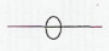
\includegraphics[width=1cm]{images/chapter3/radinstructions/01openstring.png}}$
                            & Basic indication that note to be played is not a harmonic but on open string. Recipe notation, inducement. \\
                        \textbf{2.} & ``Multiphonic''
                            & $\vcenter{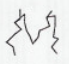
\includegraphics[width=1cm]{images/chapter3/radinstructions/02multiphonic.png}}$
                            &  Multiphonic on one string. May be modified by other glyphs. Recipe, inducement.\\
                        \textbf{3.} & ``U du `u du''---``phase shifting bow; rebouncing of the bow in between two imaginary walls; with rigid arm''
                            & $\vcenter{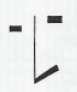
\includegraphics[width=1cm]{images/chapter3/radinstructions/03udu.png}}$
                            & Shorthand for specific body-action constraints in service of a particular indeterminate but constrained sound-field. Recipe, inducement.\\
                        \textbf{4.} & ``Little devil''---``high melody of natural harmonics (via unstable [harmonic] played with only one finger [...])''
                            & $\vcenter{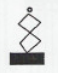
\includegraphics[width=1cm]{images/chapter3/radinstructions/04devil.png}}$
                            & (As above.)\\
                        \textbf{5.} & ``Sigma ($\Upsigma$)''---``[...] two very high but powerful simultaneous melodies of natural harmonics [...]''
                            & $\vcenter{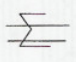
\includegraphics[width=1cm]{images/chapter3/radinstructions/05sigma.png}}$
                            & ``Second-order'' symbol modified by harmonic indications which induces complex ``micro-improvisatory'' gestures. Recipe, inducement.\\
                        \textbf{6.} & ``Alpha ($\newalpha$)''---``arpeggios of open strings [...] using very aperiodical micro rhythm''
                            & $\vcenter{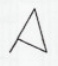
\includegraphics[width=1cm]{images/chapter3/radinstructions/06alpha.png}}$
                            & (As above.)\\
                        \textbf{7.} & ``High natural harmonics''---``high natural harmonics in LASCIAR VIBRARE [...] alternating with the open string''
                            & $\vcenter{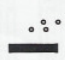
\includegraphics[width=1cm]{images/chapter3/radinstructions/07highharm.png}}$
                            & (As above.) \\
                        \textbf{8.} & Bow speed---slow
                            & $\vcenter{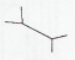
\includegraphics[width=1cm]{images/chapter3/radinstructions/08bowslow.png}}$
                            & Modifier. \\
                        \textbf{9.} & Bow speed---fast
                            & $\vcenter{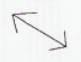
\includegraphics[width=1cm]{images/chapter3/radinstructions/09bowfast.png}}$
                            & (As above.) \\
                        \textbf{10.} & Bow pressure---flautando
                            & $\vcenter{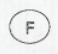
\includegraphics[width=1cm]{images/chapter3/radinstructions/10flaut.png}}$
                            & (As above.) \\
                        \textbf{11.} & Bow pressure---premuto
                            & $\vcenter{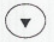
\includegraphics[width=1cm]{images/chapter3/radinstructions/11prem.png}}$
                            & (As above.) \\
                        \textbf{12.} & Phonetic rhythm---synchronous
                            & $\vcenter{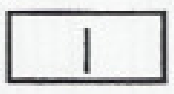
\includegraphics[width=1cm]{images/chapter3/radinstructions/12phonetic_sync.png}}$
                            & Modifier pertaining to phonetic rhythm of \textit{Tao Te Ching} inscriptions. \\
                        \textbf{13.} & Phonetic rhythm---shifted
                            & $\vcenter{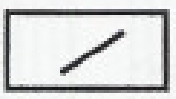
\includegraphics[width=1cm]{images/chapter3/radinstructions/13phonetic_shifted.png}}$
                            & (As above.) \\
                        \hline[0.1em]
                        \end{tblr}
                \captionsetup{width=.5\textwidth}
                \caption[Composer-provided list of symbols from Rădulescu's String Quartet No. 5 (1993), used also in \textit{Das Andere} (1984)]{Composer-provided list of symbols from Rădulescu's String Quartet No. 5 (1993), used also in \textit{Das Andere} (1984).\footnotemark}
                \label{tab:radinstructions1}
            \end{table}
                \footnotetext{\autocite{Radulescu_1993}---Instructions apply as well to the earlier \textit{Das Andere} (1984).} 
        
            \begin{table}
                \centering
                \scriptsize
                \singlespacing
                \begin{tblr}{
                    width=.7\textwidth
                    }
                    \hline[0.1em]
                    & \textbf{Glyph} & \textbf{Definition} \\
                    \hline[0.1em]
                    \textbf{1.} & F & flautando (very little pressure)\\
                    \textbf{2.} & = & normal [pressure] \\
                    \textbf{3.} & V & premuto (increased pressure) \\
                    \textbf{4.} & SP & sul ponte \\ 
                    \textbf{5.} & VP & verso il ponte (near the bridge) \\
                    \textbf{6.} & pT & un poco sul tasto \\
                    \textbf{7.} & mT & molto sul tasto \\
                    \textbf{8.} & MT & moltissimo sul tasto \\
                    \hline[0.1em]
                \end{tblr}
                \captionsetup{width=.5\textwidth}
                \caption{Additional (bespoke) modifiers given on Instruction pg. 1 of Op. 89.}
                \label{tab:radadditional}
            \end{table}

 
        \noindent Note that, like Braxton, Rădulescu uses novel symbols not only for situations which would be clumsy or entirely untenable to notate using traditional techniques, but also for greater economy in notating fairly common modifiers (flautando, sul pont., sul tasto); albeit ones which would typically be expressed in text above a staff rather than with a bespoke glyph. 
    
        Figures~\ref{fig:sigmatypical} and~\ref{fig:alphatypical} below demonstrate typical deployments of $\newalpha$ and $\Upsigma$ gestures, respectively.
            

            \begin{figure} 
                \centering
                \fbox{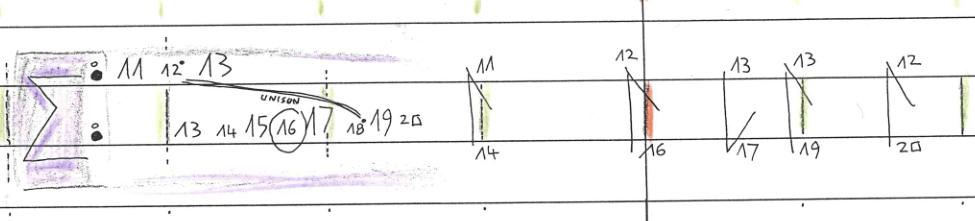
\includegraphics[width=.99\textwidth]{images/chapter3/sigma01.png}}
                \captionsetup{width=.5\textwidth}
                \caption[Typical deployment of a $\Upsigma$ figure in \textit{Das Andere}.]{Typical deployment of a $\Upsigma$ figure in \textit{Das Andere}.\footnotemark}
                \label{fig:sigmatypical}
            \end{figure}
                \footnotetext{\autocite[12]{Radulescu_1984}.}

        \noindent In Figure~\ref{fig:sigmatypical}, we find that the $\Upsigma$ spanning strings II and III is modified with a series of natural harmonic indices: 11--13 on string II and 13--20 on string III. These are not meant to be sounded ``in position' as one might expect under traditional notational syntax. Rather, these indicators provide a space for potential action; granting the performer a degree of creative latitude over the sounding events that happen at a particular time. Specifically, in what appears to be blank space on the staff, the performer is to create the aforementioned ``irregular melodies'' on both strings simultaneously using the fingering positions provided. Rădulescu helpfully provides a ``graphic simulation'' of the intended ``biphony'' between two strings on Instruction pg. 1, shown below in Figure~\ref{fig:graphicsimulation}.

    
            \begin{figure} 
                \centering
                \fbox{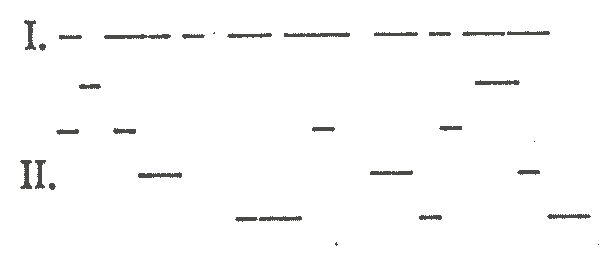
\includegraphics[width=.4\textwidth]{images/chapter3/sigmagraphicsimulation.png}}
                \captionsetup{width=.51\textwidth}
                \caption{``Graphic simulation'' of intended $\Upsigma$ biphony in \textit{Das Andere}, per Instruction pg. 1.}
                \label{fig:graphicsimulation}
            \end{figure}

    
        $\Upsigma$ modules are often interrupted by ``tick mark'' symbols featuring a single harmonic index subscript and superscript (see Fig.~\ref{fig:microclimaxes} below). These tick marks indicate, per Instruction pg. 1, ``micro climaxes'' in the continuing irregular melodies. In these instances, harmonic indices are meant to sound simultaneously for a duration proportional to the length of the glyph's ``tail,'' creating (under ideal circumstances) emergent sum and difference tones.\footnote{I can find no positive reference to the directionality of the micro-climax figures (i.e. why they sometimes appear with the ``hook'' toward the top of the staff rather than to the bottom). I suspect, from observing several performances, that it refers to the relative priority of the fingered harmonic in the climax. Similarly, the size with which $\Upsigma$ harmonic indices are printed and the presence of circled indices seem to be indicators of a desired relative prominence.}

            \begin{figure} 
                \centering
                \fbox{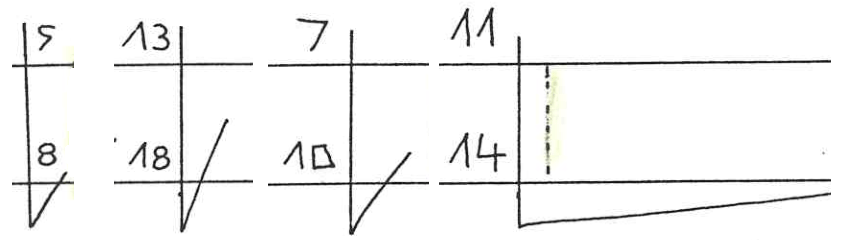
\includegraphics[width=.5\textwidth]{images/chapter3/microclimaxes.png}}
                \captionsetup{width=.5\textwidth}
                \caption[$\Upsigma$ melody micro-climaxes of various lengths in \textit{Das Andere}.]{$\Upsigma$ melody micro-climaxes of various lengths in \textit{Das Andere}.}
                \label{fig:microclimaxes}
            \end{figure}

        $\newalpha$ modules, on the other hand, encompass an entirely distinct set of gestural parameters. In lieu of a biphonic melody, each $\newalpha$ demands that a performer fill the staff's ``blank space'' with what Rădulescu calls the ``obsessive voice'' (shown with $\usym{27A1}$); involving an irregularly bowed drone on the indicated string which alternates with \textit{u du 'u du} or \textit{little devil} gestures (see Figure~\ref{fig:alphatypical} below). Here, the left hand is mostly locked in one position. Specific pitches are given at the beginning of the module which are intended to sound (albeit fragmentarily) thoughout the module. Where several pitches are indicated (as on string IV in Fig.~\ref{fig:alphatypical}), the player may transition between them at will.

        During an $\newalpha$ module, the staff is frequently cut through with wavy vertical striations which indicate rapid arpeggios. That they only ever appear upright is an indication that (like grace notes, for example) they in essence occupy no time at all on the $y$-axis. With reference to these striations, Rădulescu specifies:
    
            % arrows from fdsymbol package
            \begin{smallquote}
                The strict time distribution of the arpeggios, and the strings to which they apply [...] should be rigorously respected. Free is only:
                \begin{itemize}
                    \item the direction of the arpeggios ($\varupwavearrow$ or $\vardownwavearrow$)
                    \item the speed of their deployment, and
                    \item the point of contact along the strings. NB this should vary as much as possible but not during one bow.\autocite[Instruction pg. 3]{Radulescu_1984}
                \end{itemize}
            \end{smallquote}

            \begin{figure} 
                \centering
                \fbox{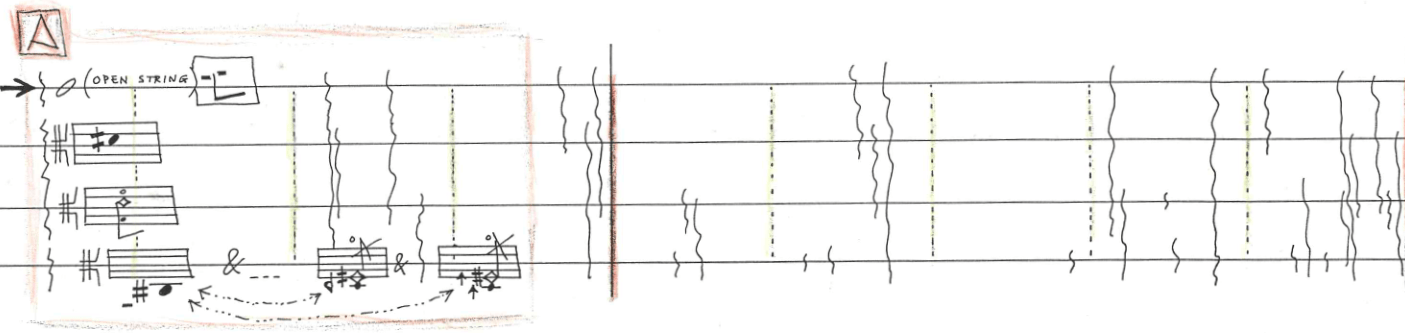
\includegraphics[width=.99\textwidth]{images/chapter3/alpha01.png}}
                \captionsetup{width=.5\textwidth}
                \caption[Typical deployment of an Alpha figure in \textit{Das Andere} with ``obsessive voice'' shown on string I.]{Typical deployment of an Alpha figure in \textit{Das Andere} with ``obsessive voice'' shown on string I.\footnotemark}
                \label{fig:alphatypical}
            \end{figure}
                \footnotetext{\autocite[4]{Radulescu_1984}.}

        \noindent Thus, the arpeggios are encoded similar to other forms of proportional notation. Given that the space between dotted vertical lines on the staff universally indicates a two-second duration, the performer must to the best of their ability map the onset of the arpeggio to its approximate location between these waypoints. Note that R\u{a}dulescu is uncommonly specific here with regard to the syntactic conventions of his novel scheme; recognizing the ambiguity of his signs and therefore specifying precisely which musical parameters remain open for creative performer intervention and which must be faithfully reproduced according to the composer's desires.

        Given their unconventional specifications and their prevalence in the score, it is worth briefly explicating the ``lesser'' combinatory gestures which often form part of $\Upsigma$ and $\newalpha$ modules. The \textit{u du `u du} and \textit{little devil} signs (3 and 4 in Table~\ref{tab:radinstructions1}) themselves serve as technique ``aggregators,'' second-order notations clustering together complexes of techniques which yield consistent but variegated and indeterminate sound. For each of these R\u{a}dulescu provides a recipe for their execution as well as a vivid verbal descriptor. \textit{U du 'u du} gestures are given formally in the score as 
        
        \begin{center}
            $\text{very fast bowing} \: (\nwsearrownew) \; F \: \& \: \pm VP \hookswarrow \!\!\! \hooksearrow mT$
        \end{center}

        \noindent indicating consistently fast and \textit{flautando} bowing with extreme variation between \textit{verso il ponte} and \textit{molto sul tasto}. He goes on to provide additional physical/gestural and sonic constraints. For instance, he mandates that the ``bowing requires a stiffly locked arm'' and that the bow should ``[change] direction very abruptly and unpredictably like the instantaneous mouvements [sic] of the Nō Theatre.'' Sonically, he specifies four important components which ought to be perceivable at all times: (1) the fundamental, (2) ``breathing noise,'' (3) ``rich variation of the harmonic content'' (4) ``an uneven `panting'-like rhythm.''\autocite[Instruction pg. 2]{Radulescu_1984} \textit{Little Devils}, to contrast, are given as

        \begin{center}
            $\text{very fast bowing} \: (\nwsearrownew) \; \pm F \: \& \: VP \leftrightarrow SP$
        \end{center}

        \noindent indicating consistently fast bowing in a narrower range between \textit{verso il ponte} and \textit{sul pont}, with fluctuation between \textit{flautando} and \textit{premuto}. As before, R\u{a}dulescu gives specific parameters for execution: the performer should ``[caress] a small part of the string in \textit{capo tasto} slowly and irregularly'' producing ``a bright and metallic sound,'' ``a cloudy phenomenon with very high register erruptions like sparklings.''\autocite[Instruction pg. 2]{Radulescu_1984}

        These signs, along with the more conventional \textit{multiphonic} and \textit{high natural harmonic} glyphs, belong to a class of symbols again basically absent from traditional notation: specifically, signs which simultaneously prescribe a particular set of physical gestures and a diffuse, uncertain resultant sound-world that nevertheless remains predictable at a larger time-scale.
        
    \subsubsection{Rădulescu's notation scheme---connotative factors}

        While R\u{a}dulescu overtly acknowledges his notation's openness by explicitly delineating certain freedoms allotted to performers in $\newalpha$ and $\Upsigma$ modules, he stops short of expressly identifying ``fixed'' and ``open'' materials as Braxton did in \textit{Composition No. 76}. As demonstrated above, the large majority of his neonotational signs are well-defined; almost to a stifling degree. Nevertheless, properly open, un-coded notation plays a subtle but important role in the \textit{Das Andere}/Op. 89 work-complex.

        Even a cursory glance at the scores of the two works reveals R\u{a}dulescu's frenetic, untamed copy-style. Both works are predominantly hand-written in the author's unpretentious print (save the title pages, \textit{Das Andere}'s instructions, and certain text in Op. 89), and no particular effort seems to have been made to keep the physical trace of the symbols consistent from page to page. To the contrary, R\u{a}dulescu's signs exhibit a sort of expressive graphicality all their own; not to the extent that it begins to inhibit legibility, but certainly to the extent that a performer might begin to interpret the symbols differently than had they been more traditionally engraved (digitally or otherwise). Though only really involving a few types of large-scale gesture, the staves often seem to display an excess of information---especially in the latter work (see, for instance, Figure~\ref{fig:radulescuexcess} below).

            \begin{figure} 
                \centering
                \fbox{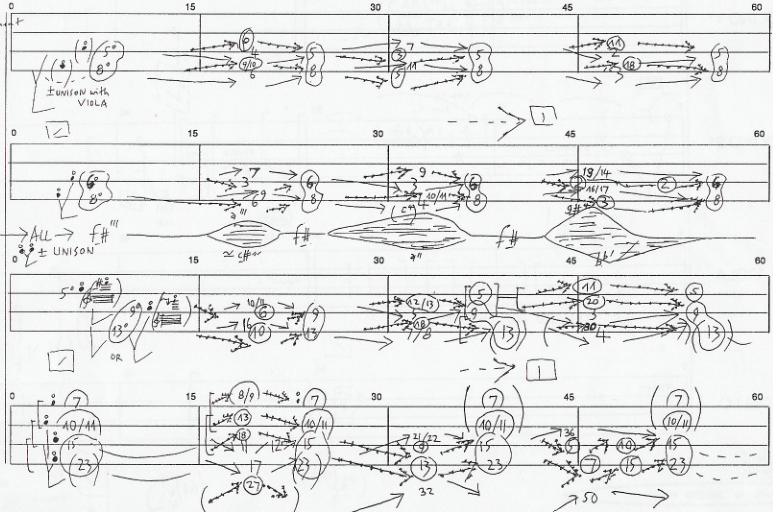
\includegraphics[width=.9\textwidth]{images/chapter3/radulescuexcess.png}}
                \captionsetup{width=.5\textwidth}
                \caption[Well-defined symbols which nevertheless demonstrate graphical ``excess'' in Op. 89.]{Well-defined symbols which nevertheless demonstrate graphical ``excess'' in Op. 89.\footnotemark}
                \label{fig:radulescuexcess}
            \end{figure}
                \footnotetext{\autocite[23]{Radulescu_1993}.}

        Featuring material outside of the primary $\newalpha$ or $\Upsigma$ gestures, the material on pg. 23 of Op. 89 functions more like a typical tablature; providing positions of natural harmonics on which performers are to place their fingers. With regard to the two types of arrows, R\u{a}dulescu gives the instruction to ``choose opposite tendencies with regards of those [sic] of your next instrument,'' indicating that performers ought to navigate the given pathways according to their neighbors' actions-in-the-moment. While these actions are all clearly-defined micro-improvisatory actions (of a sort to which the performer has by now grown accustomed), I contend that the frenzied inscription itself has a high potential to bleed through into performance; lending it a particular affect commensurate with its dense, high-energy scribble. Throughout the entire score, simple and complex information alike is presented with a similar scrawl; connoting a rapid and improvisatory compositional method.       

            % \begin{uselater}
            %     It's clear from the language in these instruction sets that Rădulescu, above all, is using notation as a sophisticated recipe to create a very particular sound world; highly indeterminate at the granular level but predictable enough that the work's formal characteristics prevail when ``zoomed out.''
            % \end{uselater}
            
        Finally, Op. 89 in particular employs text-as-notation in a particularly idiosyncratic, tricky way. The upper margin of each ``playing'' page of the score displays an excerpt from a translation of ancient Chinese poet-philosopher Lao Tzu's \textit{Tao Te Ching}. For instance:

        \begin{center}
            \LARGE
            \textsf{we work with being, but non-being is what we use}\normalsize\autocite[11]{Radulescu_1993}
        \end{center}

        \begin{center}
            \Large
            \textsf{if you want to be reborn, let yourself die}\normalsize\autocite[22]{Radulescu_1993}
        \end{center}

        \begin{center}
            \normalsize
            \textbf{\textsf{he creates confusion in those who think that they know}}
        \end{center}
        \begin{center}
            \vspace{-20pt}
            \hspace{80pt}\Huge\textsf{practice not-doing!}\normalsize\autocite[3]{Radulescu_1993}
        \end{center}
        
    
        While countless scores contain thought-provoking epigraphs and enigmatic expressive text meant to influence performance to a greater or lesser degree, R\u{a}dulescu's work is unique in that, true to form, he provides a full-page rubric on the text's interpretation (shown in Figure~\ref{fig:radulescu_triaxial} below). This rubric, taking the form of a three-axis diagram, asks that the performer ``try to realize in sound'' three clusters of interpretation-mediating factors: \{magic, symbolic \textbf{writing}, \textsc{image}\}; \{\textbf{rhythm}, phonetic spectrum, \textsc{sound}\}; \{meaning, notational communication, \textbf{idea}, \textsc{thought}\}. To be clear, despite the reference to Lao Tzu at the top of the page, I take it that these three axes are intended to hold sway over all aspects of Op. 89's interpretation---not strictly the text.
        
        \begin{figure} 
            \centering
            \fbox{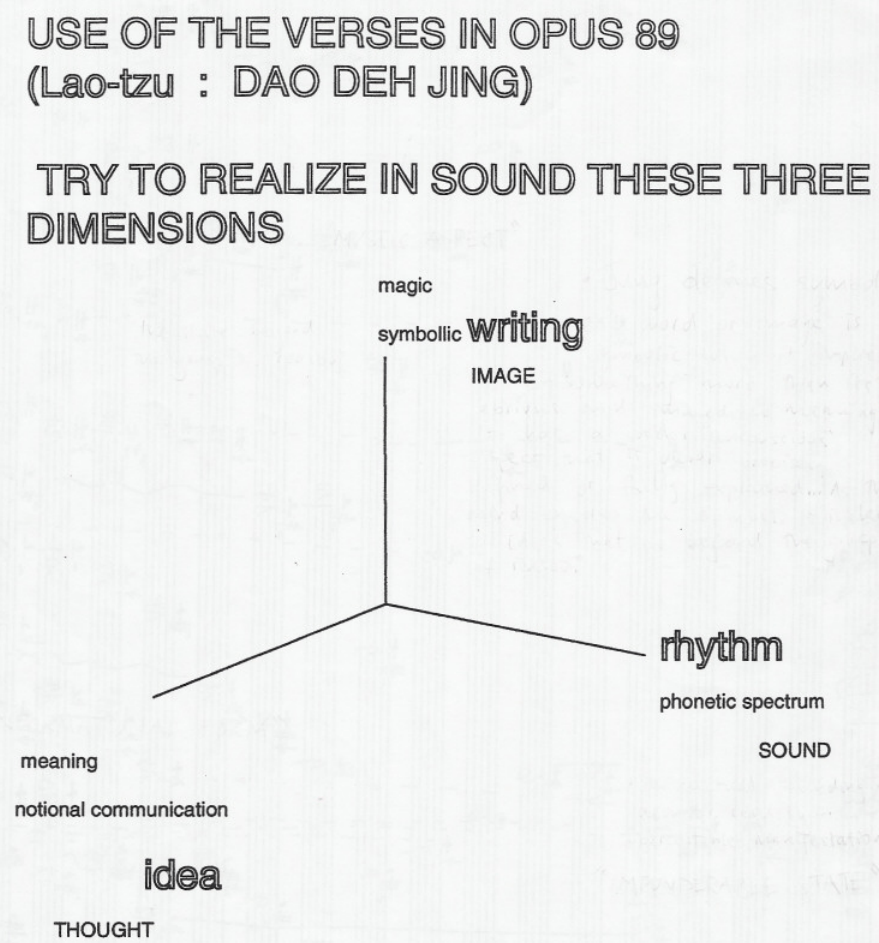
\includegraphics[width=.7\textwidth]{images/chapter3/radinstructions/radulescu_triaxial-min.png}}
            \captionsetup{width=.5\textwidth}
            \caption[Three-axis diagram representing the balancing act Rădulescu requires of the performer.]{Three-axis diagram representing the balancing act Rădulescu requires of the performer.\footnotemark}
            \label{fig:radulescu_triaxial}
        \end{figure}
            \footnotetext{\autocite[Instruction pg. 3]{Radulescu_1993}.}     
            
        The ``idea''-axis seems to be the most concrete: ``meaning'' and ``notational communication'' clearly refer to the notion that the performer should consider the concrete, denotative content of R\u{a}dulescu's glyphs---i.e. what they communicate. To ``realize [...] sound'' via this axis is to straightforwardly interpret the score according to the detailed guidelines provided. Similarly, the ``rhythm''-axis pertains to aspects of interpretation which are semi-concretely inscribed. While these phonetic/rhythmic elements are (uncharacteristically) poorly-detailed in the score's notes, William Dougherty clarifies:

        \begin{smallquote}
            The natural phonetic rhythm of these text fragments determines the rhythm of the passage below them, sometimes precisely and sometimes more impressionistically. When the symbol of a vertical line enclosed in a box is indicated, the players execute the phonetic rhythm of the text above in synch with the other players with the same symbol, while when the symbol of a (forward) slash enclosed in a box is indicated, the players execute the phonetic rhythm of the text above \textit{out of synch} with the other players. While this aspect of performance is admittedly not entirely clear from Radulescu's performance notes, an explicit example on page 13 of the score allows one to see his intent clearly [...] In this example, Radulescu actually notates the rhythm of the text -- six quavers divided into two groups of three. This corresponds to the phonetic rhythm of the text directly above, `love the world as your self'.\footnote{\autocite[37]{Dougherty_2014}.---Though Dougherty is rather detailed with regard to R\u{a}dulescu's notational practice, he neglects to speculate on the particular role that each axis of interpretation might play in performance---reducing Lao Tzu's text to its phonetic structure. His assessment here clearly refers particularly to the ``rhythm''-axis---leaving us to consider the impact of the other two.}
        \end{smallquote}

        \noindent Thus, per this axis, the text's semantic content (i.e. their meaning as used in conversational language) is entirely inconsequential. Rather, it is the phonetic makeup of the text which is to influence performance. As Dougherty explains, however, this influence is not all together straightforward. While certain (usually simpler) phrases lend themselves particularly well to the mapping process R\u{a}duescu demands (i.e. one syllable per note), far more of them require that performers find individual solutions; bespoke syllable-to-rhythm mappings.

        The third, ``writing''-axis abstracts the performer's relationship to notation to the greatest degree. To ``realize [...] sound'' in this dimension is to permit the inscriptions to act as expressive text of a particularly elusive sort. Many traditional expressive texts (\textit{espressivo}, \textit{doloroso}, \textit{con fuoco}) are so common as to verge on concrete technique indications and could thus be considered a form of denotative notation in their own right. That is to say---when a composer uses ``\textit{doloroso}'' in a score it is (unless otherwise specified) assumed that s/he intends a softer, slower performance than were it marked ``\textit{aggressivo}.'' R\u{a}dulescu's texts, however, do not afford the performer the luxury of this familiar quasi-denotative content. To allow a text like ``\textsf{the eternal void/older than GOD}''\autocite[4]{Radulescu_1993} to materially impact performance (as prescribed by the tri-axial diagram) is to engage in a particularly radical form of performer-mapping.
        
        It is worth noting here that both \textit{Das Andere} and Op. 89 eschew, for the most part, traditional expressive text proper (that is: of the form ``\textit{doloroso}'' rather than ``\textit{col legno battuto}''). The former contains a single indication to ``\textsc{\textit{[...] insist on the ``freshness'' of this g$\sharp$-spectrum}}'' on pg. 13. The latter similarly features only one indication: ``\textsc{\textit{con passione et interiorit\`{a}}}'' on pg. 5, though if the piece is to be rendered faithfully, performers of Op. 89 must maintain constant awareness of the current page's inscription and its expressive connotation. 
        
            % William Dougherty notes the uncharacteristic ``notational imprecision'' with which these textual inscriptions are placed above the material they are to influence.
        
            % \begin{notestuff}
            %     Text/graphicality of text (especially) but also of glyphs. The multiphonic notation on pg. 16 of \textit{Das Andere}. The letter of the score indicates that density and position of Alpha arpeggios is supposed to be rigorously maintained... but I'm not sure that works out in practice?
    
            %     Regardless, the ``grain'' of the notation invites (demands) a performer-mapping all its own. It's not neutrally inscribed.
    
            %     The biggest aspect, though, is the use of text and ``tri-axial'' scheme in Op. 89. Simultaneous hybridity.
            % \end{notestuff}
    
    
\section{Comparison via distinctions in notation}

        % \begin{notestuff}
        %     Where does this leave us? These are two artists who both develop bespoke notation---both undeniably ``open''. Both schemata ``traverse'' the fixed-open gradient and both prominently feature composer-mapped and performer-mapped notations---though they balance these in very different ways and they clearly do so for very different reasons. Big question: How are these REASONS reflected in the structures of NOTATION?? 
        % \end{notestuff}
    
        Having now examined, in a rather dry and pedantic way, the bare mechanics of these two distinct work-complexes, we can begin to ask more sophisticated questions regarding their composers' notational choices. In advance of that, though, it is important to take stock of precisely what we've observed. 
    
        Though the aesthetics of their inscriptions and the ways they choose to encode performer action vary greatly, there are no small number of similarities between Braxton's and R\u{a}dulescu's works. For instance, both complexes function differently from traditional ink-on-paper compositions as we've come to know them. In the last chapter I argued that for any useful definition of ``openness'' in musical composition, all works intended to be performed live by human actors are non-trivially ``open.'' It is clear, however, from our observation and listening that \textit{Composition No. 76} and \textit{Das Andere}/Op. 89 take this further; embracing openness as a core tenet of their compositional processes in a way that other, more traditional works, do not (indeed \textit{can} not given the limitations of their notational technology). This openness manifests itself both in the final sonic products resulting from the compositions' interpretation and, critically, in the way performers interpret the glyphs on the page.
        
        Both composers use a raft of symbols and other illustrations to encode their works---from commonplace to wholly alien---which vary in the extreme with regard to the degree of constraint they place upon their interpreters. In both cases, these glyphs take the form of incitements to act or sound in a particular way as well as modifiers which mediate these actions/soundings. Though these notation schemata are often startling in their graphicality, the traits listed above are on the whole not uncommon and could fairly be attributed to any number of mid-to-late-century works. Armed, however, with a more thorough understanding of the ways open notation mediates performance according to its semantic content (or lack thereof), one may begin to explore in earnest the profound gap which separates these two composers and their works. In the following section, I'll be comparing Braxton and R\u{a}dulescu along three axes: (a) the brute syntactic structure and semantic function of their adopted notation schemes in the aforementioned works, (b) the function of their notation in relation to body, process, and sound, and (c) the role that their notational choices (as regards openness) play in reflecting or articulating the tenets of their underlying philosophical frameworks.

\subsection{Traversal and hybridity}
    
        The last chapter ended with a brief elucidation of two concepts which I take to be crucial to our assessment, i.e. \textit{traversal} and \textit{hybridity}. As a brief refresher:
    
        Traversal (specifically fixed/open traversal) occurs when a system of notation is so constructed as to allow for the encoding of more-strict and less-strict instruction sets; affording narrower or broader fields of potential action to the performer, respectively. A composer who engages in traversal uses notation to tighten or loosen performance constraints over the course of a single work. This may occur gradually or suddenly or wax and wain throughout the work. Trivially, of course, traversal of this sort occurs regularly in traditional composition. Jazz compositions exhibit traversal insofar as at first, during performance of a tune's head, the performer is more tightly constrained in creative output by the ``mandatory'' recitation of the melody---then becoming less constrained during improvisation over the tune's chord changes. Likewise, a strictly notated piece of classical music might feature a section marked \textit{ad libitum} to indicate a passage involving less performer constraint. However, traversal is at its most interesting when it is deployed either for its own sake, for that of deliberately mediating the predictability/reproducibility of a musical work, or for the sake of engaging multiple distinct creative faculties of performers (as, for instance, we find in the present works). Traversal proper, as I've defined it, occurs when transitioning between symbols which are predominantly \textit{denotative}, i.e. well-defined; varying strictly in the degree to which they constrain action, not in the way they are mapped to meaning.

        Hybridity, on the other hand, (specifically connotative/denotative hybridity) occurs when well-defined symbols (mapped to meaning by convention or by the composer directly) occur alongside glyphs (or features of glyphs) which bear no fixed semantic content and must be ``manually'' mapped to meaning by the performer---either ahead of time or in-the-moment. In the last chapter, I described two types of hybridity. \textit{Concatenative} hybridity occurs when composer-mapped symbols are directly juxtaposed (spatially/temporally) on the page with strictly connotative performer-mapped glyphs. Here the performer must ``shift gears'' from the act of reading to a dual act of mapping and interpretation. \textit{Simultaneous} hybridity, to contrast, occurs when composer-mapped and performer-mapped elements are combined and must be dealt with simultaneously. Here, concrete, well defined symbols which incite action directly might be modified by performer-mapped modifiers or vice-versa. 

    \subsubsection{Traversal in \textit{No. 76}}

        \textit{Composition No. 76}'s focus on modularity lends itself to deliberate parametrization of gestural fixity by keeping its many modes of play distinct and well-defined. While there is no set order to the modules, performance often involves regular and sudden changes to the degree of constraint over potential action. Though this traversal occurs both within and between modules, (at least as regards his more fixed materials) Braxton seems to favor giving each performer a single level of gestural fixity per module. A simple example: In ``Version I'' from \textit{For Trio}, play proceeds from module pair \{J1\}--\{J2\} to \{F1\}--\{F2\} beginning at 4:44.\autocite[259]{Steinbeck_2018} Here, Player 3 moves directly from a short $\mathscr{X}$-clef system ending with a rest and quick instrument change to a system in bass clef. Given that the $\mathscr{X}$-clef (historically, at least, for Braxton) is interpreted as a melodic contour map, permitting the staff to be read ``approximately'' with any absolute pitches desired, the transition from \{J2\} to \{F1\} represents the point of traversal. This takes the form of a sudden ``squeezing'' of action potential via the addition of a single constraint: the need to observe the traditional bass clef.

            %% THESE Xes WOULD LOOK BETTER IN A MATH FONT CALLED ``EULER'' (BOLD) BUT IT SEEMS LIKE A PAIN TO IMPLEMENT SO I'M GOING TO IGNORE IT FOR NOW.
            \begin{figure} 
                \centering
                \fbox{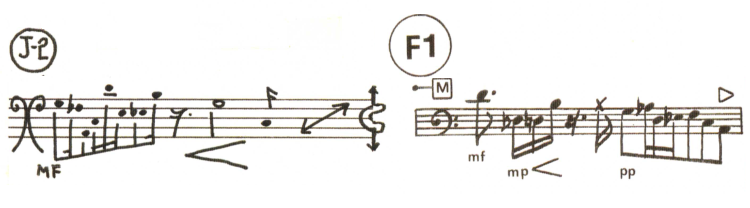
\includegraphics[width=.9\textwidth]{images/chapter3/j2f1transition.png}}
                \captionsetup{width=.5\textwidth}
                \caption{Player 3's transition from \{J2\} to \{F1\} as read in ``Version I'' on \textit{For Trio} (5'20'')}
                \label{fig:j2f1transition}
            \end{figure} 
        
        Indeed, Braxton even goes so far as to develop bespoke notational mechanisms for this fixity traversal in the form of his numeric codes accompanying improvisatory ``open'' modules.\footnote{Please forgive the continued scare-quoting of ``fixed'' and ``open'' in this section. I use these to differentiate Braxton's use of the term (to refer to his floating improvisatory sub-modules) from my own (to refer to the properties of notation at large).} Within a single module, players must regularly negotiate shifting codes attached to improvisatory inducements which flexibly constrain actions taken in response. Again in ``Version I,'' Player 1's first sub-module \{H1\} is an ``open'' one. Here, bracketing for the moment specifics of the inducements (colored shapes) themselves, Player 1 may address any of the following codes:


        \vspace{-15pt}
            \begin{align}
                [3]\:+&\:(2)\:+\:(3)---\textsc{op} \\
                \underset{\times}{(2)}\:+&\:(2)\:+\:[1]---\textsc{supp} \\
                +1\:+&\:(2)\:+\:(3)---\textsc{dom}
            \end{align}

        If, for instance, I opt to begin with the first code, the brackets surrounding numeric elements denote that my creative expression is (sequentially) constrained by (a) which little instrument I decide to use for my first three tones/phrases, (b) which (primary) instrument I use for the second two and (c) which remaining instrument I'll use for the last three. This, of course, is further mediated by the presence of the \textsc{op} code found on the attached staff-fragment indicating that my actions should be categorized ``open''---i.e. that they need not be influenced by my bandmates' actions. Executing any of these available combinations requires that the performer account for a constantly shifting network of constraints involving instrument choice, use of the voice, number of attacks, and relationship to other players.

        Gestures using fragmentary traditional/modified-traditional notation call for yet further traversal. Any time a player moves from a ``fixed'' to an ``open'' sub-module or back, he is suddenly confronted with new relational, temporal, or pitch-wise constraints which vary depending on the particular module. These constraints can be seen to change even within a given ``fixed'' gesture. Figure~\ref{fig:b1fixed} illustrates sub-module \{B1\}, in which the notes' durations are determined first by both relational and fixed parameters (whole note at a matched tempo), then by strictly relational parameters (stemless notes marked with cue arrows), then back to fixed parameters. Likewise, the phrase's dynamic is first determined collectively (the ``k'') then absolutely (\lilyDynamics{ff}).
        
             \begin{figure} 
                \centering
                \fbox{\includegraphics[width=.6\textwidth]{images/chapter3/b1.png}}
                \captionsetup{width=.5\textwidth}
                \caption{``Fixed'' sub-module B1 for Player 1 in \textit{Composition No. 76}.}
                \label{fig:b1fixed}
            \end{figure} 


            %This comes in addition to the fragmentary (modified-)traditional gestures which themselves indicate another traversal---imposing, at the very least, loose rhythm- and contour-oriented constraints (though players often opt to perform them ``verbatim''). While it is unclear whether it is mandatory that players address \textit{each} inducement in an open sub-module, players routinely switch rapidly from one to the next, each time adopting a new set of parametric constraints which apply to their improvisatory output. 

        Perhaps predictably, material in the ``fixed'' structural sequences (found after the 20 primary modules) deals with traversal in a far more disciplined manner. Here, though the base material is already considerably further open than traditional notation (with sequence 1 featuring a single-line staff and 2 featuring the diamond clef), play proceeds linearly and in unison. Only with the appearance of the ``boxed sine wave'' glyph (which, again, does not appear in any symbol key) does play break open into seemingly unconstrained improvisation with duration delimited by the next cue point.

        In sum, Braxton's large repository of well-defined symbols and codes allows notational fixity (i.e. the precise degree of constraint of player action) to be treated itself as a very finely gradated independent variable. While fixity traversal of this type is not entirely uncommon (especially among neo-notational or improv-centric works), the extent to which it suffuses \textit{Composition No. 76} and similar subsequent works is a crucial aspect of what makes Braxton's work so singular.

    \subsubsection{Traversal in \textit{Das Andere}/Op. 89}
    
        R\u{a}dulescu's traversal takes an entirely distinct form. From the first page of \textit{Das Andere}, constraints over performance are under continual flux. Unlike in \textit{Composition No. 76}, the player has no say over their assigned material at any given point in time. Rather (as with traditional notation) they must engage with each symbol as it appears, with time demarcated by dotted verticals indicating 2" durations.
        
        The opening gesture of the work, an eight-second attack on the 7th harmonic of string I, immediately gives way to a complex $\Upsigma$ gesture; an incitement to begin biphonic improvisation. In this simple traversal, the performer transitions from a field of potential with fixed finger position---ergo fixed pitch---and a narrow acceptable rhythmic accent profile to one with (constrained but) indeterminate position/pitch and more open rhythmic profile. Then, on page two (system two), R\u{a}dulescu tightens the constraints once again with a dyad on strings I and II---freezing the ``melody'' in place (see Fig~\ref{fig:datraversal} below).

            \begin{figure} 
                \centering
                \fbox{\includegraphics[width=.8\textwidth]{images/chapter3/datraversal.png}}
                \captionsetup{width=.5\textwidth}
                \caption{\textit{Das Andere}'s first three gestural territories.}
                \label{fig:datraversal}
            \end{figure} 

        Whether written in deliberately or not, the pacing of this traversal becomes an important aspect of the gestural topography of the work. Inflection points where players transition from more stringent to looser restrictions correspond fairly consistently with sonic density. Within the space of only four systems (on pages four and five), R\u{a}dulescu moves from open-melody $\Upsigma$ to more fixed $\newalpha$ (itself complicated by several optional pitches on string IV) to an entirely fixed-pitch dyad. Further, these $\Upsigma$ gestures themselves contain yet finer gradations of fixity: the simple transition from ``little devil'' to ``u du `u du'' (see Fig.~\ref{fig:datransition} below) involves also transitioning from (loosely) \{indeterminate left hand, fixed right hand\} to \{fixed left hand, indeterminate right hand\} in essentially no time at all.

            \begin{figure} 
                \centering
                \fbox{\includegraphics[width=.7\textwidth]{images/chapter3/DAtransition.JPG}}
                \captionsetup{width=.5\textwidth}
                \caption{Excerpt from \textit{Das Andere} (pg. 5, sys. 2) illustrating transition from ``little devil'' to ``u du `u du''.}
                \label{fig:datransition}
            \end{figure} 
        
        The player must not only rapidly shift between modes of sound production (as is common in all sorts of musical paradigms) but between multiple gradations of fixity in the process. This constant traversal is at the core of R\u{a}dulescu's ``micro-improvisation''---a term he uses, it seems, to refer specifically to $\newalpha$ and $\Upsigma$ environments, but which fairly applies across the entirety of both works discussed. 

        The three additional players in Op. 89 allow R\u{a}dulescu to further expand the breadth of his traversal; now encompassing inter-musician relational constraints. Like Braxton, R\u{a}dulescu uses bespoke symbols to modulate the gestures available to the symbols' interpreters; rendering these gestures contingent, realistically, on the bodily movements of one's fellow performers rather than, say, their sounds. The presence of the boxed vertical ``|,'' as mentioned above, denotes a mandatory synchrony between players' otherwise improvisatory gestures. Figure~\ref{fig:op89synchrony} below shows this technique \textit{in situ}: the second violin's micro-improvisatory \textit{lasciar vibrare} gesture is executed in a rhythm loosely dictated by the phrase at the top of the page.\footnote{\autocite[10]{Radulescu_1993}---``\textsf{can you coax your mind from its wandering and keep to the original oneness---can you cleanse your inner vision until you see nothing but the light?}''}

            \begin{figure} 
                \centering
                \fbox{\includegraphics[width=.9\textwidth]{images/chapter3/op89synchrony.png}}
                \captionsetup{width=.5\textwidth}
                \caption{Op. 89, pg. 10, second violin part demonstrating micro-improvisatory gesture modulated by relational signifiers.}
                \label{fig:op89synchrony}
            \end{figure} 

        \noindent These relational signifiers result in an FOP highly restricted in terms of finger position (natural harmonics on the specified strings only) and therefore pitch, but only loosely restricted in terms of rhythm (loosely related to the phonetic rhythm of the provided text). Indeed, as early as the second page of Op. 89 we find that R\u{a}dulescu calls for the following:

            \begin{center}
            \noindent  $\overset{\textit{very}}{\raisebox{-0.25\totalheight}{\includegraphics[width=1cm]{images/chapter3/radinstructions/13phonetic_shifted.png}}}$ - - - \textit{poco a poco} - - - $\raisebox{-0.25\totalheight}{\includegraphics[width=1cm]{images/chapter3/radinstructions/13phonetic_shifted.png}}$ - - - \textit{poco a poco} - - - $\raisebox{-0.25\totalheight}{\includegraphics[width=1cm]{images/chapter3/radinstructions/12phonetic_sync.png}}$
            \end{center}

        \noindent...that is, for a marked asynchrony of phonetic rhythms gradually transitioning to total synchrony with other players. This, in essence, directly imposes fixity traversal---this time smoothly rather than disjointedly---from a field of potential action entirely uncoupled from other players to one which requires close monitoring of their actions. To be clear, this is more significant than merely altering a single musical parameter over time (e.g. via a hairpin crescendo, etc.) in that it fundamentally restructures the performer's entire network of potential action; now made to respond to real-time factors external to the score. The player's degree of creative liberty itself is made into a manipulable variable---mediated here by these bespoke glyphs.

        To be clear, these traversal techniques are not deployed out of R\u{a}dulescu's impulse toward co-composition or to somehow meaningfully engage the generative capabilities of competent improvisers. Rather, for R\u{a}dulescu, these are simply sophisticated means of gradating the relative degree of indeterminacy at each given point in the score. Under these conditions, notational fixity becomes yet another variable (alongside global dynamic, raw sound density, density of harmonic material, etc.) which might be used to paint a dramatic arc into the structure of the work.

        % \begin{notestuff}
        %     I think this section needs some buttressing.
        % \end{notestuff}

    \subsubsection{Hybridity in \textit{No. 76}}

        Of course, these work-complexes would not merit inclusion here if it weren't for the fact that they demonstrate significant hybridity as well. To return to Braxton for a moment, \textit{Composition No. 76} seems to eschew the notion that a score must enumerate every relevant detail pertaining to its realization. As mentioned above, there are a number of ``unknowns,'' i.e., aspects of the notation's code which were evidently communicated elsewhere; deemed so self-evident as to not merit inclusion; deliberately kept opaque as an artistic decision; or simply forgotten. These omissions (which no doubt stymie any would-be Braxton analyst) highlight a critical distinction between his and R\u{a}dulescu's compositional paradigms and indeed their communities of practice as a whole. Throughout this chapter, I have, perhaps to a fault, attempted to homogenize the conceptual frameworks and terminologies used to discuss open music practices and their associated notations across both of these overlapping fields. To my mind, this allows for a no-nonsense discussion of the brute realities of the various forms of musical literacy without recourse to unnecessarily multiplied and obscurant categories of work---e.g. ``improvisatory music;'' ``indeterminate music;'' ``aleatoric music;'' ``jazz-adjacent music;'' etc. The reality of the matter, though, is that close study of this notation reveals precisely how large of an impact can be felt from the broad differences between these communities of practice.

        To gloss quickly over what is undoubtedly a fascinating and worthwhile discussion: Braxton's musical context is one which prioritizes first and foremost the ``realness of the moment''.\autocite[149]{Braxton_1988} While it would be unfair to claim that all aspects of the document are wholly negotiable, it is undeniable that unknown or ill-defined elements in the score would not pose the same moral quandary to \textit{No. 76}'s players as they would to R\u{a}dulescu's ensemble. So, while I use ``connotative,'' or ``performer-mapped'' to refer to any element that \textit{given the constraints elaborated in the score} lacks well-defined semantic content granted by the composer, I recognize that (seated in the \textit{No. 76}'s original context) these same elements may have functioned entirely differently from performance to performance depending on the demands of the situation. In the end, I take it that this flexibility and moment-centric orientation of the work strongly jibes with the dominant ethos in jazz and other Afrological improvisation paradigms which formed the core of Braxton's (and his bandmates'/co-composers') musical upbringing. This view is buttressed by close-listening to performances of \textit{No. 76}. Per Steinbeck:

            \begin{smallquote}
                Sometimes [the performers] interpret the open material rather freely instead of adhering to the notation, and these passages tend to sound more improvisatory, with fast-paced, linear melodies that depart from the steady rhythms and wide intervals of the \textit{Composition 76} score. In contrast, Braxton and his collaborators on ``Version II'' [...] typically begin with gestures derived from the notated contours, colors, and codes.\autocite[266]{Steinbeck_2018}
            \end{smallquote}

        \noindent Clearly, what constitutes faithful interpretation of the printed work in this context looks very different from what is typically considered appropriate in the Western art music paradigm. 
    
        Nevertheless, \textit{No. 76} and \textit{Das Andere}/Op. 89 now exist as works which have in some sense transcended their original context. Both scores are, at time of writing, freely available for purchase and might readily be picked up and performed entirely divorced from their initial context.\footnote{...whether or not this is well-advised is unfortunately beyond the scope of this essay.} Given that many aspects of this contextual detail are now essentially closed off except to the works' originators, we (as students of the works themselves) have no recourse but to treat these un- or incompletely-defined elements as essentially dependent on performer contribution; i.e. as ``performer-mapped'' or ``connotative'' elements.

        The colored-shape inducements featured in ``open'' improvisatory sections serve as a prime example of this tension. Lock identifies that at some point prior to \textit{No. 76}'s performance, Braxton identified a fleet of ``emotional characteristics'' ostensibly meant to modulate the piece's ``improvisation bursts'' via (in essence) a form of expressive text. However, barring discussion with Braxton himself or finding one of the few scholarly resources which detail these characteristics (never mind the problem of deciding how, precisely, to faithfully translate ``brown = complementary or harmonious or balancing'' into concrete musical terms), the aspiring performer would be left high-and-dry; only able to confront these glyphs as blank symbols waiting to be re-mapped. After all, per the text of the score, Braxton expressly grants that colors are subject to ``emotional subjective interpretation.''
    
        Therefore, delineating the boundaries of Braxton's denotative/connotative hybridity is significantly more problematic than it might be in contemporary works like Bussotti's (mentioned last chapter) in which undefined elements are squarely that: undefined. In the end, though, whether or not we bracket these issues it is clear that Braxton deliberately developed interlocking structures of denotative/connotative notation to particular ends. Whether his color scheme is interpreted as once-abstracted expressive text or as an entirely un-coded, performer-mapped subsystem, the score's interpreters, upon encountering colored materials, experience a decisive shift in the type of musical literacy they're meant to employ. Even in the case that (despite the instruction's omission from the score) we are meant to take a brown circular glyph to indicate improvisatory material which is ``complementary or harmonious or balancing,'' there is simply no fact-of-the-matter as to how these attributes are to be instantiated in sound. 

        To focus entirely on Braxton's semi-defined color scheme, however, is to ignore several other critical performer-mapped glyphs. While color is the one predominantly connotative structure which bleeds over into ``fixed'' material in the score, Braxton reserves others exclusively for his ``open'' environment. Most prominent of these is the undefined three-dimensionality which pervades the score; sometimes barely noticeable, other times extreme. Despite serving as one of the most visually arresting elements of the printed work, it seems that (unlike his use of color) Braxton never even hints at the notion that the $z$-axis is meant to materially impact performance in a controlled or rigorous way. Likewise, while Braxton explicitly references an attempt to ``integrate color and shape variables into the operational scheme of the music - as a basis to generate fresh creative responses from its instrumentalists,'' no positive rubric is given to differentiate, say, a red oval from a red quadrilateral.\autocite[143]{Braxton_1988}

        These, along with the other ``undefineds'' mentioned in the last section all point to a particular orientation toward compositional hybridity of the type defined above. Specifically, Braxton opts to integrate connotative materials of two distinct types: those which are clearly intended to be mapped and ought to have concrete sonic results (e.g. color) and those which remain fundamentally mysterious; able to be taken either as mere decoration or as a sort of notational ``excess.'' By providing these ``excess symbols'' (really, empty variables awaiting mapping), Braxton fascinatingly permits the performer to take on an even higher-level role as co-composer; deciding not only \textit{how} a graphic trace is to impact performance, but indeed whether or not a given element is to serve as notation at all.
        
          \begin{figure} 
                \centering
                \fbox{\includegraphics[width=.8\textwidth]{images/chapter3/e2e3example.png}}
                \captionsetup{width=.5\textwidth}
                \caption[Sub-modules \{E2\} and \{E3\} for Player 1.]{Sub-modules \{E2\} and \{E3\} for Player 1.\footnotemark}
                \label{fig:e2e3}
            \end{figure}
                \footnotetext{\autocite[]{Braxton_1977}.}
                
        Figure~\ref{fig:e2e3} illustrates this principle in action in sub-modules \{E2\} and \{E3\}. In \{E2\}, Player 1  reads and executes a phrase for bass clef with traditional rhythmic and dynamic constraints (with the caveat that looser reproductive constraints apply; commensurate with written works in the AACM lineage). The blue stems and noteheads, though, indicate---depending on which view one takes---either a ``sombre or moody'' coloration or some as-yet-undefined emotional affect to be mapped to blue-ness by the performer. The concurrence of well-defined traditional glyphs which induce some action and undefined notational attributes which modulate that action point to \textit{simultaneous} hybridity. Shifting to \{E3\}, however, upsets the paradigm entirely. Now Player 1 must assemble a sort of patchwork of mixed read/improvised fragments. Many elements in this pool of latent material retain familiar mappings: presumably, per the letter of the score, rhythmic indications in staff-fragments still obtain here. Alongside these denotative elements, however, are the improvisatory inducements themselves: the red oval, triangle, and quadrilateral. Though these markers are themselves modified by well-defined parameters (the numeric codes discussed in the last section), their many \textit{undefined} attributes (position in 3D-space, type of shape, point of connection to staff-fragment, mystery code) challenge the player to ascribe to (some or all of) them some distinction; sonic, gestural or otherwise. In short, to cross over from \{E2\} to \{E3\} is to enter an entirely new territory; one now characterized by the mysterious, vague, or undefined. 

        Thus, structurally, Braxton combines concatenative and simultaneous approaches to hybridity. As described earlier, Braxton himself firmly delineates what he considers ``fixed'' and ``open'' sub-modules: disjunct performance ``zones'' which loosely trace the way he opts to concatenate denotative and connotative notation. When performer-mapped symbols occur, they are typically gated-off by hard transitions; jump-cuts from one performance paradigm to another. Given that Braxton conceives of \textit{No. 76} on the whole as ``a static `dribble' of isolated events that come together and apart,'' this concatenative approach reinforces the development-less, arc-less approach the composer sought for the piece.\autocite[148]{Braxton_1988} 

        The matter is complicated, though, by Braxton's willingness to allow color (again, only semi-defined depending on what material the performer considers ``the text'' of the work) to spill over into ``fixed'' sub-modules. Here, well-defined material comprising modified traditional notation is subject to modulation via fundamentally obscure variables---a textbook case of simultaneous hybridity. Similarly, within ``open'' sub-modules, staff fragments bearing denotative content in the form of short, clefless melodies are modified by both color and some undefined position in virtual three-dimensional space. Again, coincident denotative and connotative notations require that a performer simultaneously engage in conventional reading as well as mapping when engaging with these fragments.

        To sum up: Though Braxton's use of the terms ``fixed'' and ``open'' differs considerably from common musical parlance, it is clear that he takes this division seriously. To the extent that he incorporates less-defined or undefined glyphs into \textit{No. 76}, he seems to do so according to a consistent logic corresponding to this binary distinction. Though color, shape, three-dimensionality, and (undefined) numeric code all require a considerable degree of performer-mapping in order to materially impact musical performance, Braxton opts to allow only color (the modifier closest to a form of traditional notation---namely, expressive text) to cross over into ``fixed''  material. The other elements are reserved exclusively for ``open'' sub-modules which are always (for a given player) cleanly separated spatially and temporally from material which is to be ``read.'' Nevertheless---hybridity in both its forms is a constant presence in the work; implying that mandating the performer's dual act of reading/mapping forms a critical component of the ``expanded functional and meta-functional arena'' which \textit{No. 76} creates.

    \subsubsection{Hybridity in \textit{Das Andere}/Op. 89}

        % \begin{notestuff}
        %     \begin{itemize}
        %     \item Unlike with Braxton, simultaneity is the name of the game here.
        %     \item R's use of text is very similar to B's use of color. 
        %     \item Note the discrepancy between DA and Op.89. The skeletal system was established in DA which already created sophisticated, variegated sonic surfaces via traversal. But hybridity via un-coded signs (texts) was a later addition. What motivated this change? Does the literature clarify this?
        %     \item Are there points at which the ``excess graphicality'' (i.e. decorativity?) of the notation clearly impacts performance more than incidentally? This isn't \textit{necessary} to make my point but it would help.
        %     \end{itemize}
        % \end{notestuff}

        %\paragraph{Text}
        As discussed in Section 2, undefined graphic elements(/attributes) do play a role in \textit{Das Andere}/Op. 89. However, unlike what we see in Braxton's work, R\u{a}dulescu employs a denotative/connotative hybridity which is largely the result of a single notational structure: his use of text.
    
        Throughout this chapter I've conceptually linked R\u{a}dulescu's two works on account of their many shared notational elements and their single, unifying compositional ethos (the creation of \textit{sound plasma}), referring to both of them as a single work-complex. However, if examined specifically through the lens of notational hybridity, the two works begin to look profoundly different. 

        Barring concrete indications of playing technique or brief clarifications of unfamiliar notation (\textit{G-}, \textit{D-}, or \textit{E-spectrum}; \textit{subito $\Upsigma$}; $\pm$ \textit{capo tasto}), expressive text of any sort is conspicuously absent from \textit{Das Andere}. Even within the three included pages of instructions, text is not used as a means to psychologically motivate performance, but as a highly-detailed, rather dry encyclopedia of the bespoke techniques his notation encodes. To anyone familiar with R\u{a}dulescu's quite colorful prose this might come as a surprise, especially given that well-integrated poetic text had already been a feature of his musical work for a number of years. After all, one of R\u{a}dulescu's first formal attempts at ``plasmatic'' music, \textit{Capricorn's Nostalgic Crickets} (1974, for seven identical woodwind instruments) asked performers to consider its embedded poetry ``through to its depth'' before and during performance.\autocite[9]{Marinescu}

        It seems that the intent behind \textit{Das Andere}'s conspicuous lack of poetry was the creation a sort of psychic \textit{tabula rasa}---one which allowed the piece's plasmic products to speak for themselves without the burden of being filtered through the performer's mapping scheme. In other words, \textit{Das Andere}'s radically unconventional notation and its consistent use of ``micro-improvisation'' belies the fact that the piece hews startlingly close to the traditional ``reproductive'' or ``interpretational'' paradigm of Western art music literacy. 

        This is, of course, not at all the case in the later work. Not content to deploy Lao Tzu's words as mere decoration or as ``simple'' expressive text, R\u{a}dulescu instead opts to amplify this distinctive element by rendering it in an enormous unconventional typeface; drawing the eye immediately even among dozens of novel glyphs. Where traditional expressive text might be selectively ignored or ``re-written'' to suit the demands of performance, Op. 89's text proscribes this freedom by graphically insisting upon its own relevance. The importance of text is doubly emphasized by the presence of the three-axis interpretation scheme discussed earlier. According to the rubric, text simultaneously serves both a denotative (rhythmic) and connotative (ritual) function.

        In this sense, if Braxton's work is characterized primarily by cellular, disjunct, concatenative notational hybridity, then Op. 89 is instead characterized by a radical unity of denotative and connotative elements---i.e. of simultaneous hybridity. There is, in essence, no corner of the score which is exempt from the influence of these undefined ritual elements. From beginning to end, the player must somehow contend with the \{magic, symbolic \textbf{writing}, \textsc{image}\} axis of interpretation all the while negotiating precisely-defined improvisatory tablature.

        William Dougherty's study of Op. 89, almost certainly its most comprehensive treatment, notes the relative (visual) prominence and structural importance of text in the work. In describing its function, though, he asserts that the text's ``magic'' or ritual value is entirely bound up in its rhythmic function---that these phonetic rhythms alone might ``transport the performer into a special state of awareness.''\autocite[37]{Dougherty_2014} In other words, under this view, executing the various $\newalpha$ and $\Upsigma$ gestures synchronized to phonetic rhythms itself satisfies all three axes of R\u{a}dulescu's three-dimensional rubric (Fig.~\ref{fig:radulescu_triaxial}).
        
        I would find this argument more convincing if the relationship between the text's phonetic rhythm (which is, after all, hardly obscure and easily identifiable) and the precise musical materials onto which it might conceivably map were more clear. If these rhythms themselves served as the primary ritual catalyst, I would expect their execution to be wholly unambiguous, if complex (as is the case for nearly all the rest of Op. 89's notation!). As it stands, though, R\u{a}dulescu purposefully leaves this relationship vague---precisely defining neither the phoneme/gesture interaction nor the full interpretive boundaries of the text-qua-text. 
        
        Instead, I would put forward that rhythmic interpretation of the text only fulfills one of these interpretive axes. In truth, the composer's intended holistic approach relies on multiply realizing these texts---partly (when possible) as concrete, denotative rhythmic elements, partly as gnostic expressive text onto which performers must project their own meaning. Only via this simultaneous reading/mapping---honoring both the \{rhythm\} and \{magic\} axes through notational hybridity---can the performer attain this desired ``awareness.''

        \textit{Das Andere}, entirely lacking (this particular) ritual dimension in its notation, suddenly looks like a very different piece; as though prior to the full flowering of his notation scheme R\u{a}dulescu needed to explore the possibilities of a single interpretive axis (\{notational communication\}?). The addition of connotative/denotative hybridity via ritual text (entirely lacking in \textit{Das Andere}) in the decade separating the two works amounted to an entirely new ``three-dimensionalization'' of the notation scheme.
        
        %\paragraph{Excess graphicality}

        Graphicality---i.e. notation's visual design language---is clearly an important consideration in R\u{a}dulescu's compositional methodology. Simply put, as can be seen in the many examples provided above, \textit{Das Andere} and Op. 89 demonstrate deliberate design choices which result in a very distinct, idiosyncratic notational aesthetic. These graphic parameters do not rise to the level of ``symbols'' insofar as they were not deployed to calculatedly impact performance in the same way as the many examples of neonotation which appear in the score. Nevertheless, the notation's graphic ``surface'' could be considered so striking---so alien that its graphicality might well bleed into performance practice in any case; impacting the music even outside of the nominally defined framework.

        The closest familiar parallel is probably the golden-era ``maximalist'' work of Brian Ferneyhough; a composer whose penchant for dense, thorny notation is (for better or worse) probably better known than the actual sonic trace of his music. Figure~\ref{fig:unitycapsule} below, excerpted from \textit{Unity Capsule} (1976) for unaccompanied flute, demonstrates typical Ferneyhoughian notation-density over a single $\lilyTimeSignature{2}{8}$ bar. 

            \begin{figure} 
                \centering
                \fbox{\includegraphics[width=.8\textwidth]{images/chapter3/unity-capsule-pg-14-sys-3.png}}
                \captionsetup{width=.5\textwidth}
                \caption[Excerpt from Ferneyhough's \textit{Unity Capsule} demonstrating excess graphicality (pg. 14, sys. 3).]{Excerpt from Ferneyhough's \textit{Unity Capsule} demonstrating excess graphicality (pg. 14, sys. 3).\footnotemark}
                \label{fig:unitycapsule}
            \end{figure}
                \footnotetext{\autocite[]{Ferneyhough_1976}.}
                
        Every symbol Ferneyhough uses is well-defined either by convention (in the context of late-century art music) or by the composer himself---performer-mapped ``graphic notation'' as such does not occur in his work. That is to say: a sufficiently well-programmed computer could output a meaningful rendering of each symbol precisely as it appears. However, a crucial component of Ferneyhough's work is the way that the system of notation necessarily interacts with the human element. At first glance it might seem that every conceivable aspect of performance has been parametrized and shaped by the composer's hand, thereby nullifying any creative liberties on the part of the performer. The truth, however, is that this ``information overload'' is a deliberate tack Ferneyhough takes to bring a measure of creative indeterminacy back into his work. In a mock-interview published in his \textit{Collected Writings} (1995), he asserts:

        \begin{smallquote}
            [N]otation is always relative to intention, whereby it is up to the composer to adequately suggest appropriate forms of response. [...] Given the lack of externally given criteria (historical, cultural) the composer surely has the responsibility to reflect upon such problems and to come up with forms of notation and degrees of physical involvement on the part of the performer which would begin to suggest (and then stop!) possible avenues of fruitful approach to the text. [...] One chooses degrees and emphases of notational precision with the intention of suggesting appropriate interpretational approaches to the text at hand, not with the aim of eliminating performer autonomy. Quite the opposite!\autocite[70-1]{Ferneyhough_1995}
        \end{smallquote}
        
        Stuart Paul Duncan, in an article on Ferneyhough's notational practice clarifies:

        \begin{smallquote}
            [...] Ferneyhough's music presents a map, incorporating a variety of paths in which the performer, instead of the composer, becomes the musical filter to [...] the ``world.'' In other words, the complexity of Ferneyhough's music derives not from the informational density of the score [...] ---it is not that the litany of performative instructions, upon successful completion, transparently transmits the composer's prebuilt compositional system to the listener---but rather from a coalescence of the dialogues between composer and score, score and performance, and performance and reception. \autocite[138-9]{Duncan_2010}
        \end{smallquote}

        For Duncan, Ferneyhough's notation, through its sheer density, achieves an affective graphicality which itself mediates operant composer/performer and performer/score relationships. This is accomplished by, in effect, presenting so much data that the performer has no choice but to actively filter out parameters which seem, at time of rehearsal or performance, to be less relevant than others. Ultimately, given that this filtering process is not directly guided by the composer's creative decision-making but the performer's, it constitutes a particular sort of performer-mapped openness.
        
        I take it that while he never quite matches Ferneyhough's ink-per-square-inch, the same process is at play in R\u{a}dulescu's work as well. Braxton's neo-notation is, for all its novelty, fairly comprehensible once the boundaries of play are known. Its consistency, modularity and self-pacing grant the player enough mental real-estate to both read and re-map in real time without overtaxing their creative faculties. To contrast, R\u{a}dulescu's (particularly in Op. 89) often changes drastically from page to page. Micro-improvisational inducements will appear in multiple forms, either with specific modifiers or without. Often the page will become cluttered with arrows, ties and slurs, tiny or extremely large instructions in differing scripts, branching paths, clarifications of clarifications, etc. Where Ferneyhough's notation was painstakingly engraved (each note copied with a calligraphic pen or hand-rubbed from the beautiful---now sadly extinct---Notaset dry-transfer paper), R\u{a}dulescu's spindly copy-style seems itself wild and improvisatory---commensurate with the rapid-fire shifting between playing techniques. Compounded by the complexity of the aformentioned text, all of these factors combine to yield a dense network of material; never literally \textit{impossibly} dense, but intricate at least to the extent that precise constraints over the performer's potential action must be mapped, in part, by the performers themselves.

\subsection{How does (open) notation serve the artist?}

    The above analysis shows how two very different composers, armed with sophisticated, bespoke neo-notation schemata, achieve familial but quite distinct performance environments, ultimately serving very different compositional goals. In this section, I would like to briefly assess the ways in which the structure of these schemata are able to support these goals and how two types of (what might broadly be considered) ``open notation'' are able to achieve radically distinct---in some ways even antithetical---effects.

    To grossly oversimplify a complex topic: We might reduce the driving force behind R\u{a}dulescu's oeuvre to the creation, by various means, of a single sonic-ritual phenomenon---\textit{sound plasma}. \textit{Das Andere} and Op. 89 are by no means the only two works to achieve this goal. Rather, they represent a local point of refinement of R\u{a}dulescu's process; a point at which the composer had developed an entire bespoke notation scheme for efficient \textit{sound plasma} production. Roger Heaton describes this mysterious \textit{sound plasma} in an article from 1983 (note: the year prior to \textit{Das Andere}'s premiere).

        \begin{smallquote}
            Radulescu's works are built from sound situations created by different treatments of fundamentals, the spectra produced by these treatments, and the isolation of individual spectra. The music results `naturally' from the initial organisation of sound sources and formal structures, its interest lying in the interaction of the resulting harmonics, difference tones, subtones, rhythmic beats, and so on. The texture thus produced is called the `sound plasma';
            \begin{quote}
                there are no longer steps, interval jumps, chords etc., but discreetly gliding and trembling narrow frequency bands, vibrating (living) sound plasma. [...] Hence, rhythm exists no longer as combined values, but only as spectrum pulse of the micro and macro sound plasma [...]\autocite{Radulescu_1975}
            \end{quote}
            To put it simply, the ways in which the global sound sources are treated must follow certain `compositional' laws if their product is to fuse together and achieve `the sound micro and macro plasma, as the real music of the future'.\autocite[23-4]{Heaton_1983}
        \end{smallquote}

    Though neither \textit{Das Andere} or Op. 89 mention the term explicitly, the phenomenon Heaton describes fits their resultant sound-worlds perfectly. What R\u{a}dulescu does give us is a rather enigmatic description of his goals in particular with \textit{Das Andere}:

        \begin{smallquote}
            This music, at the border between score and sound phenomenon, is trying to create a state of trance, close to a spiritism seance where we would invoke our own \textit{alter ego} or \textit{anti-I}. The sole subconscious ``register incline'' might render conceivable the advent of that psycho-acoustical phantom due to the continuous spectral enrichment of the instrument in its low. \autocite[dedication page]{Radulescu_1984}
        \end{smallquote}

    Thus, we might assume, R\u{a}dulescu designed \textit{Das Andere}'s notation so as to bring about \textit{sound plasma}'s sonic and ritual properties as efficiently as possible given the instruments (and instrumentalists) with whom he intended to work. Ritual considerations, after all, must still abide by real-world pressures such as rehearsal time, musician hourly rates, etc. As such, he has taken string-specific gestural parameters (bow speed, bow pressure, bow position, left hand placement and rate of movement) and clustered them together into mutable, flexible second-order symbols ($\newalpha$, $\Upsigma$, etc.) which, through the use of a number of modifiers, finely regulate the performers' micro-improvisatory movements. This, in turn, allows the performer to quickly grasp the otherwise devilishly complex ``body data'' needed to produce \textit{sound plasma} to R\u{a}dulescu's satisfaction.

    Here the composer has solved two problems at once: (1) Where users of neo-notation are often faced with the prospect of memorizing the function of dozens of new symbols; in effect forcibly reconfiguring their entire network of notational affordances, R\u{a}dulescu has deployed comparatively few new symbols and has taken care to organize them logically according to function. In addition, several of these symbols replicate functions already present in traditional notation; further diminishing the learning curve for their adoption. (2) By making each of these second-order symbols flexibly modifiable by common-sense parameters (the positions of natural harmonics accompanying $\Upsigma$ gestures, for instance), he has ensured that these symbols gestural domains---i.e. the fields of potential they afford players---are sufficiently detailed, with a high degree of variability. That is to say: one symbol, properly configured, might result in an entire galaxy of sounds.

    \textit{Das Andere}'s notation, in short, was developed primarily because it was the most straightforward means of achieving this difficult, arcane sound-world; side-stepping the need for walls of explanatory or expressive text or a dense jungle of 32nd-note figures which would never succeed in capturing the ``emergent'' properties of \textit{sound plasma} anyway. As it happens, the quickest way to this goal is the direct manipulation of the body---a notational action-map comprising bodily processes rather than sonic events.

    We understand what Martin Suckling means when he describes R\u{a}dulescu's notational practice as requiring ``near-continuous improvisation'' and ``open[ing] a door [to] the performer's creativity.''\autocite[2]{Suckling_2018} Certainly there is an extent to which the performer's ``creative'' rather than ``reproductive'' faculties must be engaged when performing this music. For instance, the precise contour of the harmonic melody performed in $\Upsigma$ modules is up to the whim of the player---as are ``the direction of the arpeggios [...], the speed of their deployment, and the point of contact along the strings'' in the $\newalpha$ modules.\autocite[Instruction pg. 3]{Radulescu_1984} However, closer inspection reveals that collaborative interplay (perhaps the first thing we think of when encountering the term ``improvisation'') is in fact the furthest thing from R\u{a}dulescu's mind. Rather, this notation marks an attempt to radically decouple the performer from his/her creative faculties by engaging precise, raw body-data rather than more traditional or more open, improvisational forms of notation---``[forcing] performers to think differently than they do when playing conventional music, ensuring a fresh interpretation that is fee of many preconceived parameters of traditional playing technique.''\autocite{Dougherty_2014} This is an open notation which renders the player's years- or decades-old muscle memory and cognitive maps obsolete, and which acts not as a call to create, but as a detailed (albeit indeterminate) instruction manual for the creation of \textit{sound plasma}. 

    By this point it will have become clear that in some ways, Braxton's and R\u{a}dulescu's systems (and motivating ideologies) bear more than just a passing resemblance. Both are artists wholly oriented toward creating music for the future---music which by its very structure points the way forward for all manner of artistry and for society as a whole. Various denotative and connotative forms of notation and their attendant fixity traversal and hybridity represent important tools in both composers' arsenals with which they intend to bring about their world-transforming artworks. Both artists work (to use the eternal present tense) in dogged pursuit of certain musical ideals which they envision lasting long after their own passing.

    However, where R\u{a}dulescu seeks, through notation, to take direct control of the performer's bodily gestures in service of a divine, gnostic sound-world, Braxton takes a very different approach. For one, Braxton employs a much larger library of symbols, which tend to focus not on entabulating the parameters of the body, but on invoking improvisatory utterances featuring varying constraints. Braxton's approach to notation in \textit{No. 76} is not that of an artist with a unified notion of a particular sound-world seeking the most efficient instruction set to bring it about. Rather, Braxton orients his composition around a sophisticated \textit{process} which acts as a musico-philosophical beacon toward future art-making; one which necessarily draws in many distinct aspects of human creativity.
    
    To return to a topic glossed in the last section: In his 1985 philosophical \textit{magnum opus} the \textit{Tri-Axium Writings}, Braxton himself broadly addressed what he took to be critical distinctions between Euro- and Afrological orientations toward musical notation.
    
    \begin{smallquote}
            The use of notation in creative improvised music has yet to be really examined in all its different permutations. For the reality of this consideration functions on several levels which are outside of European art music. Notation as practiced in black improvised creativity is not viewed as a factor that only involves the duplication of a given piece of music - and as such an end in itself. Rather this consideration has been utilized as both a recall-factor as well as a generating factor to establish improvisational coordinates. In this context notation is utilized as a ritual consideration and this difference is important for establishing the reality platform of the music - dictating the harmonic and rhythmic sound-path of activity and also as a center factor. [...]
    \end{smallquote}

    \noindent In other words, notation in the Black improvised music tradition functions less as a means of bringing about an idealized, museum-grade reproduction of an honored work of art, and more as a device to aid in musical ``recall'' and ``generation.'' A piece of music by a great tune-writer which is subsequently transcribed into lead-sheet format is a vehicle for creativity; the use of which constitutes a type of musical ritual. He continues:

    \begin{smallquote}
            \noindent For to experience the music of any creative orchestra is to see the re-shifting of structural and vibrational moment-events [...] as a means to have the fixed-activity of a given composition re-ordered to deal (or apply) with the physical universe particulars of its performance. Today the use of re-ordering in this manner is called alienatory [sic] or indeterminism - but this practice has been utilized in creative music from the black aesthetic since its inception. Notation in this context invariably becomes a stabilizing factor that functions with the total scheme of the music rather than a dominant factor at the expense of the music. [...]

            \vspace{7pt}
            
            \noindent The fact is - western art music has come to only utilize its functionalism with respect to the dynamics of re-interpretation [...] and in no way does the dynamics of interpretation compare of [sic] the freedom inherent in the functional arena of creative black music.\autocite[35-7]{Braxton_1985}
        \end{smallquote}

    \noindent For Braxton, notation which brings about indeterminate gesture or sound is part and parcel of the Black improvisatory project---its ``rediscovery'' and renaming by European or New-York-School composers in the 1950s is immaterial. However, Braxton's own project was always more ambitious than would be allowed by a single Afro- or Eurological musical vantage point. Traditional notation as wielded by the great mid-century improvisers by itself would prove insufficient to bring about Braxton's real goals: the establishment of a truly trans-idiomatic form of music-making. Per Braxton's explicit ``mission statement'' given in the \textit{Composition Notes}:

    \begin{smallquote}
        [...] this composition was not designed to adhere to either the current misconceptions surrounding the word `jazz' (with respect to how the science of that thrust is viewed, or so-called viewed - in this time zone) nor can this work be defined in `western art music' terms. Rather the meta and empirical foundation of this work was conceived with respect to the spiritual and composite vibrationatory affinity-area of world culture.\autocite[136-7]{Braxton_1988}
    \end{smallquote}

    It is only fitting, then, that this ``composite'' music-making paradigm reveal itself to its participants via a similarly composite notation system. Braxton's scheme, in its ``fixed'' sub-modules, draws in the flexible fixity of ``Afrological'' lead-sheet performance. Melodies presented here are ``fixed'' in the same sense that a standard's melody is fixed in jazz performance; that is, in such a way that it might undergo creative transformation all the while retaining some persistent, recognizable identity in each of its realizations. However, Braxton clearly borrows, in equal measure, modes of play which originated with American and/or European scored open musics. ``Collage-able,'' order-agnostic musical modules (both at the macro- and micro-scale) clearly hearken back to the early experiments with open notation which Eco identified in \textit{The Open Work}; Stockhausen's \textit{Klavierstück XI}, for instance, which represented an early example of modular notation organized according to the performer's whim.\autocite[1]{Eco_Robey_1989} Likewise, his experiments with alternative clefs reflect notations which prioritize melodic contour over specific pitch set (as in Andriessen's \textit{Workers Union} (1975) from a few years prior). Critically, certain elements appear \textit{sui generis} where no suitable subsystem existed from which to borrow. Braxton needed bite-sized improvisatory ``outbursts,'' but ones which might be modulated, filtered, rendered contingent at a moment's notice. While many solutions existed, Braxton opted to incorporate color, shape, numeric code, and three-dimensionality; all factors which were already present to one degree or another in his long-running creative metasystem.

    Instead of beginning with a complex imagined sound-world and carefully selecting the most economical notation scheme to bring it about, Braxton in effect ``composes'' a finely-tuned system (via what I've called a \textit{process-concept}) comprising various forms of musical literacy, interactivity, creative constraint, ``emotional subjective interpretation,'' etc., in order to ultimately bring about his desired third-millennium form of Ur-creativity. While his notation frequently constrains performers' sonic outputs via the usual means (choice of instrument, melodic contour, rhythmic parameters, etc.), the creative process is the real locus of Braxton's composerly intent.

    We might sum up the creative differences between the two composers thus (see Fig.~\ref{fig:flowdiagram} below):

    \begin{figure}
        \centering
            \scalebox{0.75}{\begin{tikzpicture}[->,>=stealth',shorten >=1pt,auto,node distance=2cm,ultra 
                                    thick,main node/.style={circle,draw,minimum size=2cm}] %,font=\rmfamily\small\bfseries
                \node[main node, label=above:\textit{\textbf{Comp. No. 76}}] (a) {\textsc{notation}};
                \node[main node, fill=red!30] (b) [below = of a] {sound};
                \node[main node, fill=cyan!30] (c) [below = of b] {process};
                \node[main node, fill=blue!30] (d) [below right =2cm and 3cm of c] {body};
                \node[main node, label=above:\textbf{\textit{Das Andere}}] (e) [right =5cm of a] {\textsc{notation}};
                \node[main node, fill=blue!30] (f) [below = of e] {body};
                \node[main node, fill=red!30] (g) [below = of f] {sound};
                \node[main node, fill=cyan!30] (h) [below right =2cm and 3cm of g] {process};
                \path[every node/.style={font=\rmfamily\small}]
                (a) edge node [fill=white, anchor=center, pos=0.5] {designed to influence} (b)
                (b) edge node [fill=white, anchor=center, pos=0.5] {to achieve a certain} (c)
                (c) edge node [fill=white, anchor=center, pos=0.5, rotate=55] {incidentally impacting} (d)
                (e) edge node [fill=white, anchor=center, pos=0.5] {designed to influence} (f)
                (f) edge node [fill=white, anchor=center, pos=0.5] {to achieve a certain} (g)
                (g) edge node [fill=white, anchor=center, pos=0.5, rotate=55] {incidentally revealing} (h);
            \end{tikzpicture}
            }
        \captionsetup{width=.5\textwidth}
        \caption{Illustration of influence ``flow'' through \textit{Composition No. 76} and \textit{Das Andere}}
        \label{fig:flowdiagram}
    \end{figure}

    Of course, R\u{a}dulescu complicates this reading by expanding \textit{Das Andere}'s notation scheme to encompass a distinctly Braxtonian ``subjective interpretation'' during the construction of Op. 89. \textit{Das Andere}, written nine years prior, had already put forward a more-or-less complete vehicle for the creation of \textit{sound plasma} even without provisions for performer-mapped notational semantic content. Though the factors which transmuted body-data into ``precisely imprecise'' sound remained essentially unchanged between the two works, R\u{a}dulescu saw fit to expand the ritual function of the music---taking it from a mere downstream effect of the sound to an inseparable aspect of the act of performance itself. At this point it becomes particularly difficult to ignore the extent to which R\u{a}dulescu's three-axis interpretation rubric (Fig.~\ref{fig:radulescu_triaxial}) echoes Braxton's now-venerable Tri-Axial philosophy (for which his philosophical tract was named) which suffuses all aspects of his creative expression.\footnote{Unfortunately, this work lacks the space for a full (or even modest) rendering of the central tenets of Braxton's Tri-Axial philosophy. For now it must suffice to explain that Braxton conceives of his work as drawing together many crucial sets-of-threes: \textit{mutable}, \textit{stable}, and \textit{correspondence} logics (traditional improvisation, extant works, open works); ritual and performance logics of the past, present, and future; the \textit{primary}, \textit{secondary}, and \textit{tertiary} material of Ghost Trance Music; the three levels of inquiry used to construct the \textit{Tri-Axium Writings} (which are, of course, separate from the three central \textit{goals} of the \textit{T-AW}: \textit{affinity postulation}, \textit{axium correlation}, and \textit{reality imposition}). --- For more information, please see \shortcite{Braxton_1985}; \shortcite{Cauwenberghe_2021}; \shortcite{SA16}; \shortcite{Lock_1989}; \shortcite[167-75]{Lock_2000}; \shortcite{Lock_2008}}
    
    While the existence of a direct lineage between the two conceptual frameworks is unlikely, it seems noteworthy (to say the least!) that R\u{a}dulescu's effort to create new forms of notation (intended specifically to represent the music's ritual considerations) manifested itself in a three-dimensional structure directly homologous to Braxton's own tri-axial artwork-interpretation (etc.) scheme. In expanding \textit{Das Andere}'s notation to include Lao Tzu's sacred/secular text as well as an appropriate set of tools to bring it to bear on Op. 89's sonic materials, R\u{a}dulescu integrates multi-layered structures of denotative/connotative notational hybridity in much the same way Braxton had nearly two decades prior. Rather than interpret this change as a sudden realignment of R\u{a}dulescu's musical priorities, we might read the ``three-dimensionalization'' of the \textit{Das Andere} system not as a means of replacing but of \textit{reemphasizing} the music's spiritual component; an aspect already present but in danger of being lost if the work was only ever a series of micro-improvisatory physical gestures and the whirling, buzzing sound-world they produced. R\u{a}dulescu's music never sought to reach the same diversity of macro- and micro-level improvisatory play-environments that Braxton created in \textit{No. 76}. In deploying his unique mode of simultaneous hybridity, however, R\u{a}dulescu was able to, at least fractionally, allow his performers to play a collaborative role in ascertaining the shape and color of the \textit{sound plasma} ritual.
    
    \section{Conclusion}

    \textit{Prima facie}, the two compositional paradigms elaborated over the past fifty or so pages seem fairly similar. Both artists begin with essentially the same sorts of raw materials:

    \begin{smallquote}
    \begin{itemize}
        \item a foundation in traditional notation;
        \item a need to create a particular sort of indeterminate sound-world;
        \item a system of ``graphic'' open notation featuring...
        \begin{itemize}
            \item well-defined elements for inducing action and modifying that action and
            \item more vaguely-defined or un-defined elements requiring performer-mapping to function;
        \end{itemize}
        \item and a notational syntax which contextualizes these elements and allows their spatio-temporal deployment.
    \end{itemize}
    \end{smallquote}

    Further, both artists blend traditional and bespoke notations; making for a playing experience in which musicians must balance traditional notions of recitation with active creative decision-making through forms of improvisation. Readily apparent, however, to anyone with even a passing knowledge of these artists is that their compositional processes, their musical products, and their attendant philosophical frameworks differ wildly. The paradox articulated by this distinction---namely ``How do two work-complexes, both nominally neo-notational and improvisatory, wind up so vastly different?''---is one I hoped to begin answering in this chapter. Specifically, it has been my contention that more subtlety exists in the ways novel systems of notation are constructed and used than is typically addressed in scholarly literature. Deeper understanding of the ways that notation serves to mediate performance (and performer/composer agencies) demands a more thorough mode of interrogation---not only of general properties of notation systems (as we found in Ligeti's novel typology last chapter), but of the specific ways that new notations are lent meaning in the context of a musical work. 

    Braxton and R\u{a}dulescu strike me as two of our most fascinating systems-developers. Throughout their respective catalogues (though perhaps especially in the works mentioned here), both demonstrate dogged pursuit of (truly) radical musical ideals and both share an expertise in the way notation can be used to bring these ideals to bear for both performer and listener. I hope that this chapter has served not only as a justification for my admiration of these artists' working methods, but also as an elucidation of the ways notation's fundamental particles can dramatically influence compositional systems. I contend that only through a greater understanding of notation's general operating principles---e.g. through efforts like Ligeti's novel notation typology established last chapter---as well as close examination of these notational quanta, that we might more fully come to terms with notation's power and influence over the way we write and perform music.

    % \begin{notestuff}
    %     But in bringing them together and eschewing any one level of creative engagement with the written material, Braxton does something truly unique. His point is to explore human creativity in all of its forms and under all sorts of creative constraints; something none of his predecessors really accomplished. Notation is an excellent mechanism to achieve this.
    % \end{notestuff}

    % \begin{notestuff}
    %     Though 76 was written well before these ideas were cemented in prose, its score exemplifies the ideals of the Afrocentric orientation toward notation Braxton describes here. [then describe the process mentioned last paragraph as exemplifying this]
    % \end{notestuff}

    % \begin{notestuff}
    %     \begin{itemize}
    %         \item Braxton's context is one of improv-first. Everything is negotiable and subject to change according to (to use his term) the ``realness of the moment.''
    %         \item Rad's context is one in which undefineds or unknowns are typically critical errors---which demand immediate rectification lest the performance be less-than-complete or less-than-authentic.
    %         \item I am using the term ``connotative'' or ``performer-mapped'' to refer to anything that (GIVEN THE CONSTRAINTS LAID OUT IN THE SCORE) lacks well-defined semantic content granted by the composer. 
    %         \item There is a sense, though, in which (given the hyper-negotiable nature of the score) anything and everything is subject to change, to re-mapping at the performer's whim. 
    %         \item In this sense Braxton's ``hybridity'' is then, absolute, since nearly everything is both decisively denotative and apt to be re-mapped.
    %         \item Nevertheless, these works are now functionally autonomous. Contemporary performers who pick these works up and intend to perform them are not privy to the ``private details'' pertaining to notation interpretation which may have been known quantities in the work's initial context.
    %         \item Therefore we have no choice but to go ahead and treat the unknown and ill-defined elements as essentially open to performer-mapping; ergo a critical part of the structures of hybridity present in the work.
    %     \end{itemize}
    % \end{notestuff}

    % \paragraph{R\u{a}dulescu} While the subtlety with which R\u{a}dulescu traverses structures of indeterminacy is itself noteworthy, it is worth examining separately the way that un-coded, strictly connotative structures seep into his otherwise rigorous system. 

